\chapter{KMOS Observations in NGC\,6822}
\label{ch:ngc6822}
% \begin{figure}
%  \centering
% \centering
% \subfloat[Science One caption]{
\includegraphics[width=0.65\textwidth]{ngc6822/figure1}}
% \subfloat[Science Two caption]{
\includegraphics[width=0.65\textwidth]{ngc6822/figure2}}
% \caption[Short caption]{A long and descriptive caption about the two subfigures included above.}
% \label{fig:figures1+2}
% \end{figure}

% \section{Section One}

% \begin{table}
% \centering
% \caption{An example table, illustrating the use of the booktabs package.}
% \begin{tabular}{cccc}
% \toprule
% Here & is & a & table \\
% \midrule
% 1 & 2 & 3 & 4 \\
% 5 & 6 & 7 & 8 \\% \bottomrule
% \end{tabular}
% \label{tab:example}
% \end{table}


\section{Introduction}

\label{sec:introduction}
A promising new method to directly probe chemical abundances in external galaxies is with $J$-band spectroscopy of red supergiant (RSG) stars.
With their peak flux at
$\sim$~1\,$\mu$m and luminosities in excess of
10$^4$\,L$_\odot$, RSGs are extremely bright in the near-IR,
making them potentially useful tracers of the chemical abundances of star-forming galaxies out to large distances.
To realise this goal,
\cite{2010MNRAS.407.1203D} outlined a technique to derive metallicities of RSGs at moderate spectral resolving power
($R$~$\sim$~3000).
This technique has recently been refined using observations of RSGs in the Magellanic Clouds
\citep{2015ApJ...806...21D} and Perseus OB-1
\citep{2014ApJ...788...58G}.
Using absorption lines in the $J$-band from iron, silicon and titanium, one can estimate metallicity
([Z]~=~log\,Z/Z$_{\odot}$) as well as other stellar parameters
(effective temperature, surface gravity and microturbulence) by fitting synthetic spectra to the observations.
Owing to their intrinsic brightness,
RSGs are ideal candidates for studies of extragalactic environments in the near-IR.

To make full use of the potential of RSGs for this science, multi-object spectrographs operating in the near-IR on 8-m class telescopes are essential.
These instruments allow us to observe a large sample of RSGs in a given galaxy, at a wavelength where RSGs are brightest.
In this context, the $K$-band Multi-Object Spectrograph
\citep[KMOS;][]{2013Msngr.151...21S} at the Very Large Telescope (VLT), Chile, is a powerful facility.
KMOS will enable determination of stellar abundances for RSGs out to distances of $\sim$~10\,Mpc.
Further ahead, a near-IR multi-object spectrograph on a 40-m class telescope, combined with the excellent image quality from adaptive optics,
will enable abundance estimates for individual stars in galaxies out to tens of Mpc,
a significant volume of the local universe containing entire galaxy clusters
\citep{2011A&A...527A..50E}.

Here we present KMOS observations of RSGs in the dwarf irregular galaxy NGC\,6822,
at a distance of $\sim$~0.46\,Mpc
\citep[][and references therein]{2012AJ....144....4M}.
Chemical abundances have been determined for its old stellar population
\citep[e.g.][]{2001MNRAS.327..918T,2013ApJ...779..102K},
but knowledge of its recent chemical evolution and present-day abundances is
somewhat limited.
Observations of two A-type supergiants by
\cite{2001ApJ...547..765V} provided a first estimate of stellar abundances, finding
log\,(Fe/H)~+~12~=~7.01$\pm$0.22 and
log\,(O/H)~+~12~=~8.36$\pm$0.19, based on line-formation calculations for these elements
assuming local thermodynamic equilibrium (LTE).
A detailed non-LTE study for one of these objects confirmed the results finding
$6.96\pm 0.09$ for iron and $8.30\pm0.02$ for oxygen
\citep{2002PhDT.........3P}.
Compared to solar values of 7.50 and 8.69, respectively
\citep{2009ARA&A..47..481A},
this indicates abundances that are approximately one third solar in NGC\,6822.
A study of oxygen abundances in H\,\2 regions
\citep{2006ApJ...642..813L} found a value of $8.11\pm0.1$, confirming the low metallicity.

NGC\, 6822 is a relatively isolated Local Group galaxy, which does not seem to be associated with either M31 or the Milky Way.
It appears to have a large extended stellar halo
\citep{2002AJ....123..832L,2014ApJ...783...49H}
as well as an extended HI disk containing tidal arms and a possible HI companion
\citep{2000ApJ...537L..95D}.
The HI disk is orientated perpendicular to the distribution of old halo stars and has an associated population of blue stars
\citep{2003MNRAS.341L..39D,2003ApJ...590L..17K}.
This led \cite{2006ApJ...636L..85D} to label the system as a ``polar ring galaxy''.
A population of remote star clusters aligned with the elongated old stellar halo have been discovered
\citep{2011ApJ...738...58H,2013MNRAS.429.1039H}.
In summary, the extended structures of NGC\,6822 suggest some form of recent interaction.

In addition, there is evidence for a relatively constant star-formation history within the central 5\,kpc
\citep{2014ApJ...789..147W}
with multiple stellar populations
\citep{2006A&A...451...99B,2012A&A...540A.135S}.
This includes evidence for recent star formation in the form of a known population of massive stars, as well as a number of H\,\2 regions
\citep{2001ApJ...547..765V,2006AJ....131..343D,2009A&A...505.1027H,2012AJ....144....2L}.

In this chapter I present near-IR KMOS spectroscopy of RSGs in NGC\,6822 to investigate their chemical abundances.
In Section~\ref{sec:observations} the details of the observations are described.
Section~\ref{sec:data_reduction} describes the data reduction and
Section~\ref{sec:results} details the derived stellar parameters and investigates the spatial distribution of the estimated metallicities in NGC\,6822.
A discussion of the key results is presented in Section~\ref{sec:discussion} and
Section~\ref{sec:conclusions} concludes the chapter.

% section introduction (end)

\section{Observations}
\label{sec:observations}

\subsection{Target Selection} % (fold)
\label{sub:target_selection}

Targets were selected from optical photometry
\citep{2007AJ....134.2474M}, combined with near-IR ($JHK{_s}$) photometry
\cite[for details see][]{2012A&A...540A.135S} from the Wide-Field Camera (WFCAM) on the United Kingdom Infra-Red Telescope (UKIRT).
The two catalogues were cross-matched and only sources classified as stellar in the photometry for all filters were considered.

Our spectroscopic targets were selected principally based on their optical colours, as defined by
\cite{1998ApJ...501..153M} and
\cite{2012AJ....144....2L}.
Figure~\ref{fig:BVR} shows cross-matched stars, with the dividing line at
$(B - V)$~=~1.25~$\times (V - R)$~+~0.45.
All stars redder than this line, above a given magnitude threshold and with
$V - R >$~0.6, are potential RSGs.

Distinguishing between RSGs and the most luminous stars on the asymptotic giant branch
(AGB) is difficult owing to their similar temperatures and overlapping luminosities.
Near-IR photometry can help to delineate these populations,
with RSGs located in a relatively well-defined region in the near-IR ($J-K$) colour-magnitude diagram (CMD), as discussed by
\cite{2000ApJ...542..804N}.
The near-IR CMD from the WFCAM data is shown in
Figure~\ref{fig:JK} and was used to further inform our target selection.
Employing the updated CMD criteria from
\cite{2014A&A...562A..32C}  -- modified for the distance and reddening to NGC\,6822 --
all of our potential targets from the combined optical and near-IR criteria are (notionally) RSGs.


The combined selection methods yielded 58 candidate RSGs, from which 18 stars were observed with KMOS, as shown in Figure
\ref{fig:N6822}.
The selection of the final targets was defined by the KMOS arm allocation software {\sc karma}
\citep{2008SPIE.7019E..0TW},
where the field centre was selected to maximise the number of allocated arms,
with priority given to the brightest targets.
Optical spectroscopy of eight of our observed stars, confirming them as RSGs, was presented by
\cite{2012AJ....144....2L}.


\begin{figure}
 \centering
 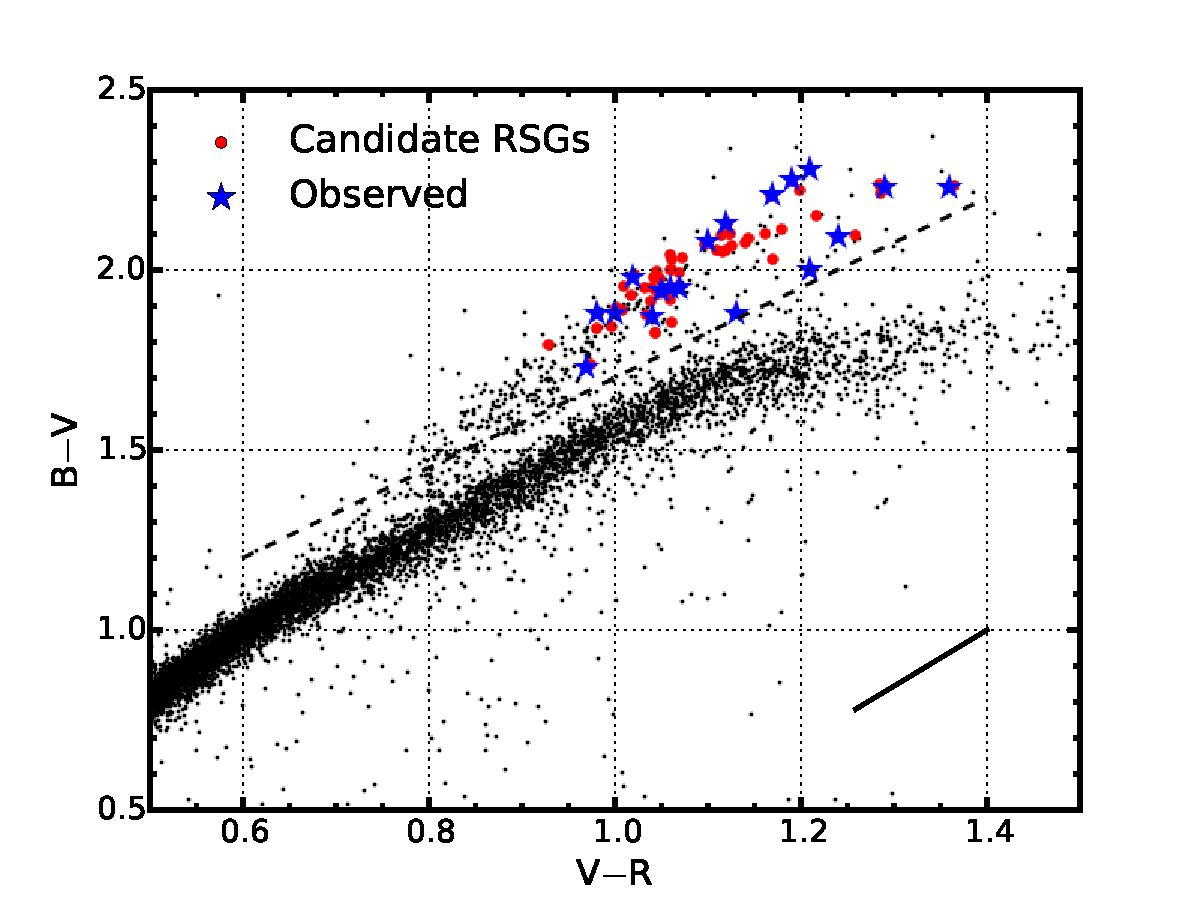
\includegraphics[width=0.65\textwidth]{ngc6822/N6822_bvr}
 \caption[$B-V$ against $V-R$ two colour diagram]{
          Two-colour diagram for stars with good detections in the optical and near-IR photometry in NGC\,6822.
          The black dashed line marks the selection criteria using optical colours, as defined by
          \protect\cite{2012AJ....144....2L}.
          Red circles mark all stars which satisfied our selection criteria.
           % and our $J$-$K$, $K$ cut.
          Large blue stars denote targets observed with KMOS.
          The solid black line marks the foreground reddening vector for $E(B-V)$~=~0.22
          \protect\citep{1998ApJ...500..525S}.
         }
 \label{fig:BVR}
\end{figure}

\begin{figure}
 \centering
 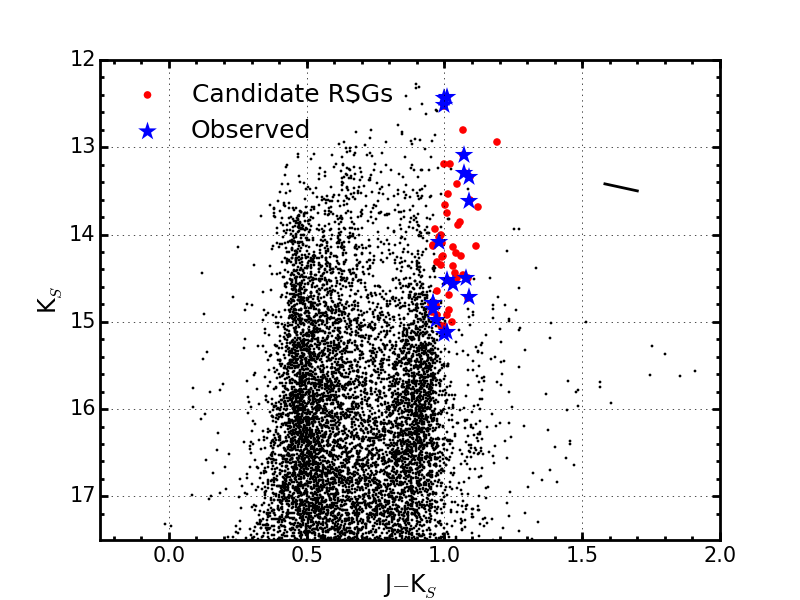
\includegraphics[width=0.65\textwidth]{ngc6822/N6822_jk}
 \caption[$J-K$ colour magnitude diagram]{
          Near-IR colour-magnitude diagram (CMD) for stars classified as stellar sources in the optical and near-IR catalogues, plotted using the same symbols as Figure~\ref{fig:BVR}.
          This CMD is used to supplement the optical selection.
          The solid black line marks the foreground reddening vector for $E(B-V)$~=~0.22
          \protect\citep{1998ApJ...500..525S}.
          % The green solid box indicates the region defined by
          % \protect\cite{2014A&A...562A..32C} as containing supergiants.
         }
 \label{fig:JK}
\end{figure}


\begin{figure}
 \centering
 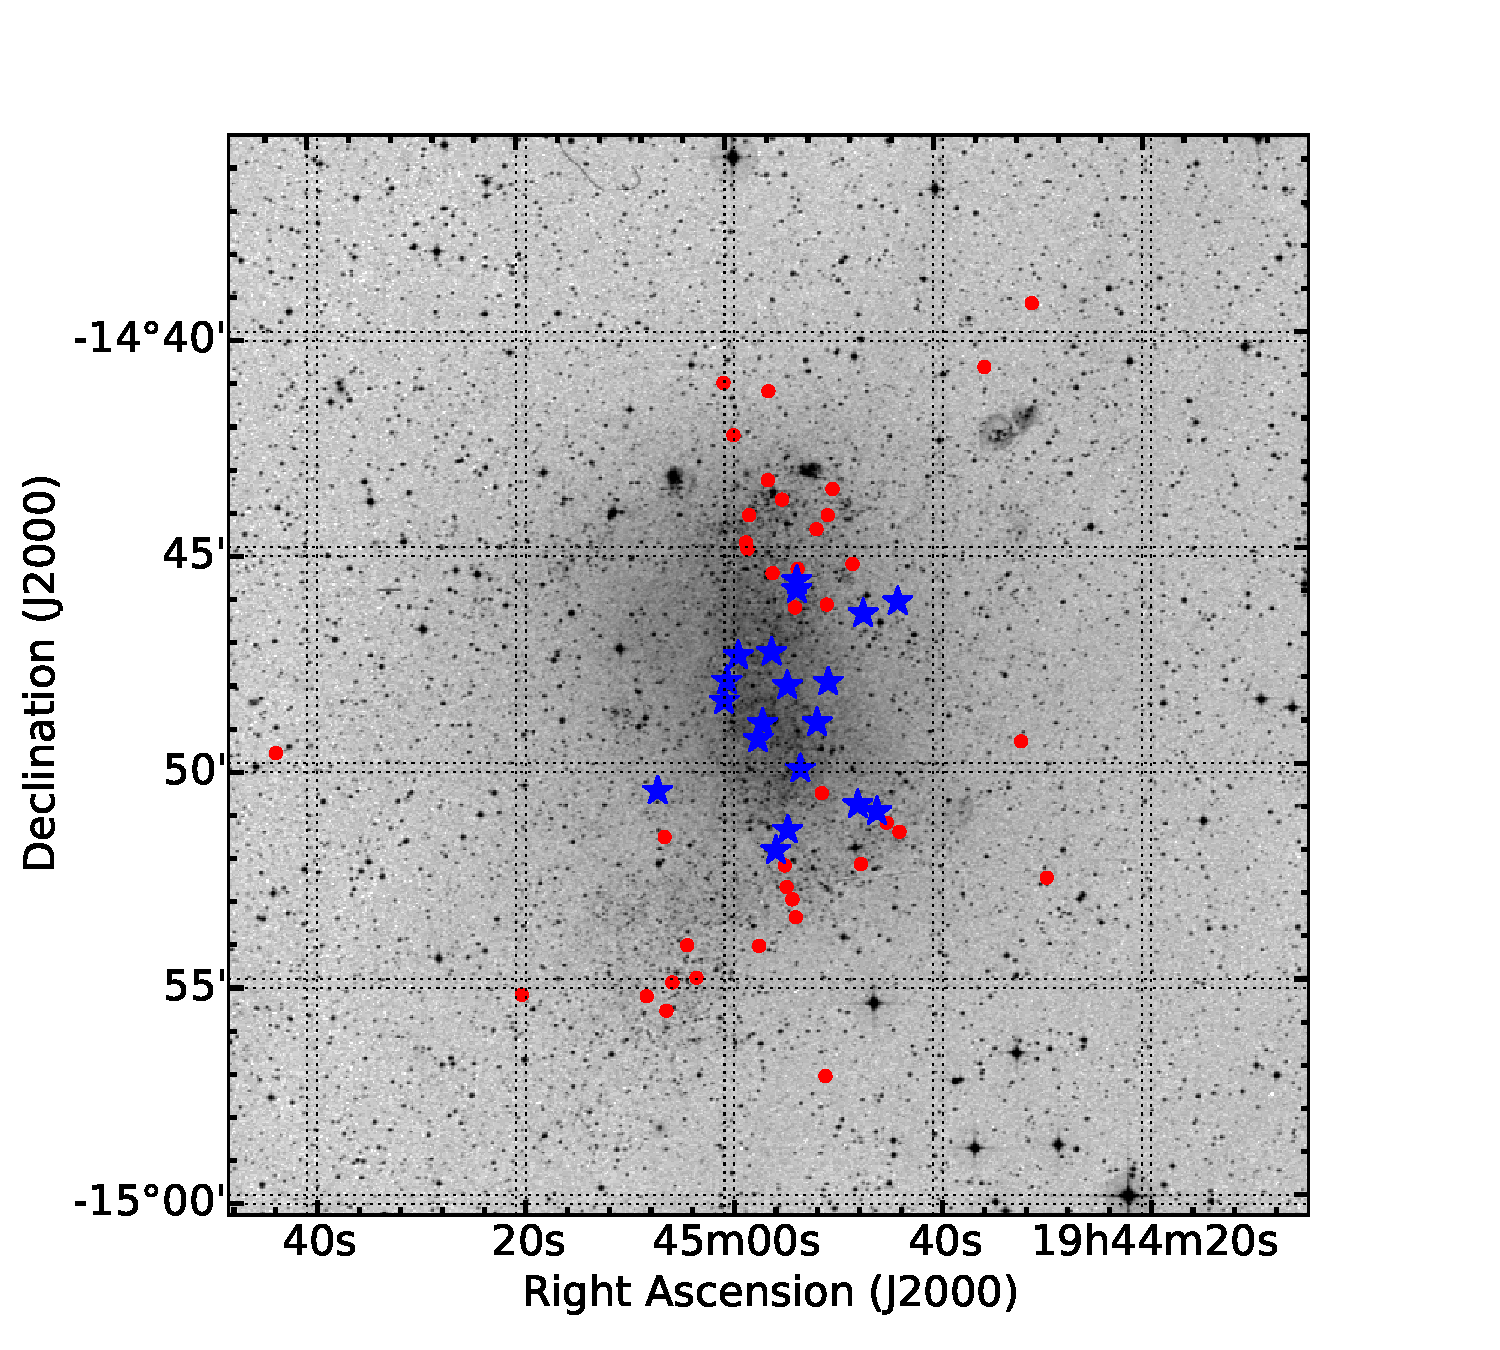
\includegraphics[width=0.65\textwidth]{ngc6822/N6822_RSGs_thesis}
 \caption[Targets identified in on-sky image]{Spatial extent of the KMOS targets over a Digital Sky Survey (DSS) image of NGC\,6822.
          Blue stars indicate the locations of the observed red supergiant stars.
          Red filled circles indicate the positions of red supergiant candidates selected using out photometric criteria (see Section~\ref{sub:target_selection}).
          }
 \label{fig:N6822}
\end{figure}

% section target_selection (end)

\subsection{KMOS Observations} % (fold)
\label{sub:observations}

The observations were obtained as part of the KMOS Science Verification program on 30 June 2013 (PI: Evans, 60.A-9452(A)),
with a total exposure time of 2400\,s
(comprising 8\,$\times$\,300\,s detector integrations).
% Observations for this study are from the new KMOS instrument on the VLT, Chile.
KMOS has 24 deployable integral-field units (IFUs) each of which covers an area of
2\farcs8 $\times$ 2\farcs8 within a 7\farcm2 field-of-view.
The 24 IFUs are split into three groups of eight, with the light from each group relayed to different spectrographs.
KMOS is described in more detail in \textbf{Chapter x.x}.

Offset sky frames
(0\farcm5 to the east) were interleaved between the science observations in an object (O), sky (S) sequence of:
O,\,S,\,O,\,O.
This observing sequence was chosen over a more standard O\,S,\,O sequence to increase time spent on science objects.
The observations were performed with the $YJ$ grating
(giving coverage from 1.02 to 1.36$\mu$m);
estimates of the mean delivered resolving power for each spectrograph (obtained from the KMOS/esorex pipeline for two arc lines) are listed in Table~\ref{tb:res}.

In addition to the science observations, a standard set of KMOS calibration frames were obtained consisting of dark, flat and arc-lamp calibrations (with flats and arcs taken at six different rotator angles).
A telluric standard star was observed with the arms configured in the science positions, i.e. using the {\em KMOS\_spec\_cal\_stdstarscipatt} template in which the standard star is observed sequentially through all IFUs.
The observed standard was HIP97618, with a spectral type of B6\,III
\citep{1988mcts.book.....H}.

A summary of the observed targets is given in
Table~\ref{tb:obs-params}.
A signal-to-noise (S/N) ratio of $>~100$ per resolution element is required for satisfactory results from this analysis method
\citep[see][]{2014ApJ...788...58G}.
We estimated the S/N ratio of the spectra by comparing the counts in the brightest spatial pixels
(within the 1.15-1.22$\mu$m region) of each source with the counts in equivalent spatial pixels in the corresponding sky exposures
(between the sky lines).
The S/N estimated is knowingly an underestimate of the true S/N achieved.

% \footnotetext{http://www.usm.uni-muenchen.de/people/wegner/kmos/en/karma.php}

\begin{table*}
\caption{Measured velocity resolution and resolving power across each detector.\label{tb:res}}
\scriptsize
\begin{center}
\begin{tabular}{crcccc}
\hline
\hline
Det. & IFUs & \multicolumn{2}{c}{Ne\,\lam1.17700\,$\mu$m}
            & \multicolumn{2}{c}{Ar\,\lam1.21430\,$\mu$m} \\
 & & FWHM [\kms] & $R$ & FWHM [\kms] & $R$ \\
  \hline
1 & 1-8 &  \a88.04\,$\pm$\,2.67 & 3\,408\,$\pm$\,103 &
           \o85.45\,$\pm$\,2.67 & 3\,511\,$\pm$\,110 \\
2 & 9-16 & \a82.83\,$\pm$\,2.48 & 3\,622\,$\pm$\,108 &
           \o80.30\,$\pm$\,3.05 & 3\,736\,$\pm$\,142 \\
3 & 17-24 & 103.23\,$\pm$\,2.73 & 2\,906\,$\pm$\,77\a &
            101.25\,$\pm$\,2.99 & 2\,963\,$\pm$\,87\a \\
\hline
\end{tabular}
\end{center}
\end{table*}

\begin{sidewaystable}
\caption[Summary of VLT-KMOS targets in NGC\,6822]{Summary of VLT-KMOS targets in NGC\,6822.\label{tb:obs-params}}
\scriptsize
\begin{threeparttable}
\centering
\begin{tabular}{lrcccccccccl}
 \hline
 \hline
ID & S/N & $\alpha$ (J2000) & $\delta$ (J2000) & $B$ & $V$ & $R$ & $J$ & $H$ & $K_{\rm s}$ & RV (\kms) & Notes \\
 \hline
NGC6822-RSG01 & 223 &   19:44:43.81  &  $-$14:46:10.7  &  20.83  &  18.59  &  17.23  &  14.16  &  13.37  &  13.09  &  $-$63.8$\pm$3.2 & Sample\\
NGC6822-RSG02 & 120 &   19:44:45.98  &  $-$14:51:02.4  &  20.91  &  18.96  &  17.89  &  15.53  &  14.72  &  14.52  &  $-$60.6$\pm$5.5 & Sample\\
NGC6822-RSG03 &  94 &   19:44:47.13  &  $-$14:46:27.1  &  21.30  &  19.41  &  18.41  &  16.13  &  15.35  &  15.12  &  $-$69.8$\pm$6.5 \\
NGC6822-RSG04 & 211 &   19:44:47.81  &  $-$14:50:52.5  &  20.74  &  18.51  &  17.22  &  14.37  &  13.58  &  13.30  &  $-$65.5$\pm$4.4 & LM12 (M1), Sample \\
NGC6822-RSG05 & 104 &   19:44:50.54  &  $-$14:48:01.6  &  20.83  &  18.95  &  17.97  &  15.75  &  14.98  &  14.79  &  $-$74.8$\pm$5.0 \\
NGC6822-RSG06 & 105 &   19:44:51.64  &  $-$14:48:58.0  &  21.33  &  19.45  &  18.32  &  15.81  &  14.95  &  14.72  &  $-$65.3$\pm$6.0 \\
NGC6822-RSG07 & 145 &   19:44:53.46  &  $-$14:45:52.6  &  20.36  &  18.43  &  17.38  &  15.06  &  14.30  &  14.08  &  $-$53.8$\pm$5.1 & LM12 (M4.5), Sample \\
NGC6822-RSG08 & 103 &   19:44:53.46  &  $-$14:45:40.1  &  20.88  &  19.14  &  18.17  &  15.95  &  15.16  &  14.98  &  $-$51.6$\pm$4.1 & LM12 (K5), Sample \\
NGC6822-RSG09 & 201 &   19:44:54.46  &  $-$14:48:06.2  &  20.56  &  18.56  &  17.35  &  14.43  &  13.67  &  13.34  &  $-$47.4$\pm$2.1 & LM12 (M1), Sample\\
NGC6822-RSG10 & 302 &   19:44:54.54  &  $-$14:51:27.1  &  19.29  &  17.05  &  15.86  &  13.43  &  12.66  &  12.42  &  $-$75.7$\pm$3.5 & LM12 (M0), Sample \\
NGC6822-RSG11 & 327 &   19:44:55.70  &  $-$14:51:55.4  &  19.11  &  16.91  &  15.74  &  13.43  &  12.70  &  12.43  &  $-$59.3$\pm$4.0 & LM12 (M0), Sample \\
NGC6822-RSG12 & 100 &   19:44:55.93  &  $-$14:47:19.6  &  21.43  &  19.56  &  18.52  &  16.14  &  15.33  &  15.14  &  $-$39.2$\pm$4.6 & LM12 (K5) \\
NGC6822-RSG13 & 106 &   19:44:56.86  &  $-$14:48:58.5  &  21.05  &  19.06  &  18.04  &  15.81  &  15.05  &  14.85  &  $-$55.7$\pm$7.4 \\
NGC6822-RSG14 & 284 &   19:44:57.31  &  $-$14:49:20.2  &  19.69  &  17.41  &  16.20  &  13.52  &  12.76  &  12.52  &  $-$84.2$\pm$1.9 & LM12 (M1), Sample \\
NGC6822-RSG15 & 124 &   19:44:59.14  &  $-$14:47:23.9  &  21.30  &  19.17  &  18.05  &  15.58  &  14.74  &  14.50  &  $-$86.9$\pm$6.6 \\
NGC6822-RSG16 & 107 &   19:45:00.24  &  $-$14:47:58.9  &  21.27  &  19.20  &  18.10  &  15.60  &  14.80  &  14.57  &  $-$67.7$\pm$3.1 \\
NGC6822-RSG17 & 167 &   19:45:00.53  &  $-$14:48:26.5  &  20.84  &  18.75  &  17.51  &  14.70  &  13.86  &  13.61  &  $-$64.8$\pm$4.2 & Sample\\
NGC6822-RSG18 & 104 &   19:45:06.98  &  $-$14:50:31.1  &  21.06  &  19.12  &  18.06  &  15.74  &  14.94  &  14.78  &\a$-$33.8$\pm$11.7& Sample\\
\hline
\end{tabular}

\begin{tablenotes}
  \item Optical data from
  \protect\cite{2007AJ....134.2474M}, with typical photometric uncertainty 0.016, 0.006, 0.010 in $B, V$ and $R$ bands respectively.
  Near-IR data from the UKIRT survey
  \protect\cite[see][for details]{2012A&A...540A.135S}, with typical errors 0.015, 0.010, 0.012, in $J, H$ and $K$ bands respectively.
  Targets observed by
  \protect\cite{2012AJ....144....2L}
  are indicated by \textquoteleft
  LM12\textquoteright~ in the final column (with their spectral classifications in parentheses).
  Targets used for abundance analysis are indicated by the comment
  \textquoteleft Sample\textquoteright
  .
\end{tablenotes}
\end{threeparttable}
\end{sidewaystable}


% subsection KMOS observations (end)
% section observations (end)

\section{Data Reduction} % (fold)
\label{sec:data_reduction}

The observations were reduced using the recipes provided by the Software Package for Astronomical Reduction with KMOS
\citep[SPARK;][]{2013A&A...558A..56D}.
The standard KMOS/esorex routines were used to calibrate and reconstruct the science and standard-star data cubes as outlined by
\cite{2013A&A...558A..56D}.
Sky subtraction was performed using the standard KMOS recipes and telluric correction was performed using two different strategies.
Throughout the following analysis all spectra have been extracted from their respective data cubes using a consistent method (i.e. the optimal extractions within the pipeline).

\subsection{KMOS/esorex pipeline} % (fold)
\label{sub:kmos_esorex_pipeline}

The KMOS/esorex pipeline performs the initial calibrations by using a set of dark, flat and arc-lamp calibrations.
These calibrations are all performed on raw KMOS images which contain 14$\times$14 spectra from each IFU from the three spectrographs.
The flat-field calibrations allow one to trace the spatial coordinates of each spectrum on the raw images.
This information is then combined with the wavelength calibration information,
obtained from the arc-lamp calibrations, to give a 14$\times$14$\times$2056 3-D spectrum for each IFU across the detector.
A snapshot of the 14$\times$14 spatial pixels is shown in Figure~\ref{fig:IFU_snapshot}.
When reducing multiple exposures of a single object, this cube is then combined to produce the final data cube.

There are many routines with which to extract spectra from this final data cube.
The simplest way to do this is to take the single brightest spectral pixel within the cube and extract a spectrum from that.
However, higher signal-to-noise can be achieved by extracting the spectrum from a circular pixel mask centred on the brightest pixel, where each pixel is weighted by the integrated flux in that pixel.
However, within each IFU, the resolution of the spectrum varies between spatial pixels.
Therefore, in order to combine the spectra more precisely, one must first standardise the resolution across the IFU before combining~\citep{2015ApJ...805..182G}.

% subsection kmos_esorex_pipeline (end)

\subsection{Sky Subtraction} % (fold)
\label{sub:sky_subtraction}

Sky subtraction is performed within the pipeline before IFU reconstruction where the science frame is matched with its nearest in time sky frame.
Initial inspection of the extracted stellar spectra revealed minor residuals from the sky subtraction process.
Reducing these cases with the \textquoteleft sky\_tweak\textquoteright
~option within the KMOS/esorex reduction pipeline was ineffective to improve the subtraction of these features.
Any residual sky features could potentially influence our results by perturbing the continuum placement within the model fits, which is an important aspect of the fitting process
\citep[see][for more discussion]{2014ApJ...788...58G,2015ApJ...806...21D}.
Thus, pending a more rigorous treatment of the data
(e.g. to take into account the changing spectral resolution across the array),
we exclude objects showing sky residuals from our analysis.
Of the 18 observed targets, 11 were used to derive stellar parameters
(as indicated in Table~\ref{tb:obs-params}).

\subsubsection{In-house Sky Subtraction} % (fold)
\label{sub:in_house_sky_subtraction}

An alternative method of sky subtraction would to to subtract the sky from spatial pixels within the object IFU.
This is possible as within each IFU the target does not extend over the entire set of spatial pixels as Figure~\ref{fig:IFU_snapshot} demonstrates.
Using a collection of these spatial pixels which contain little or no object flux can be a potential method for sky subtraction.
Clearly this method has large potential benefits with respect to observing efficiency as less sky exposures would be needed for a given observing run.
Theoretically, the sky subtraction from a region which is nearer in space to the object in question is beneficial in two different ways:
\begin{enumerate}
  \item The sky being subtracted more closely represents the sky background which the object is contaminated with.
For comparison, during the sky exposures the telescope is offset by $\sim$~10 arc-minutes, therefore, this sky exposure samples an intrinsically different atmospheric column when compared to the science exposure.
Even though the differences in the sky lines on this spatial scale is small, as the signal originating from the sky is roughly an order of magnitude larger than that of our object, a small sky residual could affect the shape and/or strength of a genuine stellar feature.
% Quantify this!
\item The region of the host galaxy which the target object occupies will often contain contaminating flux.
By sampling a region of space closer to the position of the target object, the underlying galaxy flux will be more accurately subtracted.
\end{enumerate}

However, an inherent issue with this method of sky subtraction is that one may well remove some of the object flux in this process.
Additionally, (as mentioned in~\ref{sub:kmos_esorex_pipeline}) there is know to exist a slight difference in resolution over the spatial extent of the IFU which could make comparisons between spatial pixels complicated.
By standardising the resolution across the IFU one can potentially obtain a more reliable sky subtraction at the expense of the resolution of the spectrum.


\begin{figure}
 \centering

\includegraphics[width=0.55\textwidth]{ngc6822/N6822_RSG17-snapshot}
 \caption[IFU Snapshot]{
          Snapshot of a reconstructed KMOS IFU (at $\lambda$~=~1.16\,$\mu$m) containing the science target NGC6822-RSG17.
          Darker shades indicate higher flux.
          This image serves to demonstrate that the target objects do not entirely fill the KMOS IFU.
          This therefore, presents the possibility for using several pixels which do not contain flux from the object in the sky subtraction process.
          }
 \label{fig:IFU_snapshot}
\end{figure}

  % subsection in_house_sky_subtraction (end)

% subsection sky_subtraction (end)
\subsection{Telluric Correction} % (fold)
\label{sub:telluric_correction}

One of the most important stages within the data reduction process for spectroscopic observations from ground-based observatories concerned with measuring absorption, rather than emission, features is the correction for the effects of the Earth's atmosphere.
As starlight passes through the atmosphere it is absorbed and re-emitted by various different molecules.
These strong molecular features contaminate and blend genuine stellar features.
In order to recover the stellar features a spectrum is derived which contains only the atmospheric absorption features.
This spectrum is then used to correct the science spectrum.
% To illustrate this I could show a plot of the transmission model in the near-IR

Typically, one generates a telluric spectrum by observing an additional star of known spectral type.
If the stellar features are well characterised for this spectral type, any additional features are assumed to be owing to the Earth's atmosphere.
The spectral type is usually chosen to minimize the number of stellar features present in the region of interest.
In the $J$-band an A0V star has few lines of note and is therefore a good choice of telluric standard star in this regime.
% Show a plot of an A0V star in the near-IR
This method of telluric correction is robust and well tested and is the preferred method for many different studies.
However, it does have some fairly fundamental limitations which include the fact that it is impossible to sample precisely the same atmospheric column in both the science and telluric observations, as well as the additional time it takes to observe a standard star.

Recently, a tool for telluric correction which does not require standard star observations has been developed and tested on some VLT instruments~\citep{2015A&A...576A..77S}.
This package uses atmospheric modelling techniques to derive a telluric spectrum.
The package is briefly explained in section~\ref{sub:molecfit},
however, see~\citet{2015A&A...576A..77S} for a more thorough description.


% subsection telluric_correction (end)

\subsection{Three-arm vs 24 arm Telluric Correction} % (fold)
\label{sub:three_arm_vs_24_arm_telluric_correction}

The default template for telluric observations with KMOS is to observe a standard star in one IFU in each of the three spectrographs.
However, there is an alternative template which allows users to observe a standard star in each of the 24 IFUs.
This strategy should provide an optimum telluric correction for the KMOS IFUs but reduces observing efficiency.

A comparison between the two methods in the $H$-band was given by
\cite{2013A&A...558A..56D},
who concluded that using the more efficient three-arm method was suitable for most science purposes.
However, an equivalent analysis in the $YJ$-band was not available.
To determine if the more rigorous telluric approach is required for our analysis,
we observed a telluric standard star (HIP97618) in each of the 24 IFUs.
This gave us the data to investigate both telluric correction methods and to directly compare the results.

We first compared the standard-star spectrum in each IFU with that used by the pipeline routines for the three-arm template in each of the spectrographs.
Figure~\ref{fig:IFU_compare} shows the differences between the standard-star spectra across the IFUs,
where the differences in the $YJ$-band are comparable to those in the $H$-band
\cite[cf. Fig.7 from][]{2013A&A...558A..56D}.
The qualitative agreement between the IFUs in our region of interest (1.16-1.22$\mu$m) is generally very good.


\begin{figure*}
 \centering
 \begin{center}
 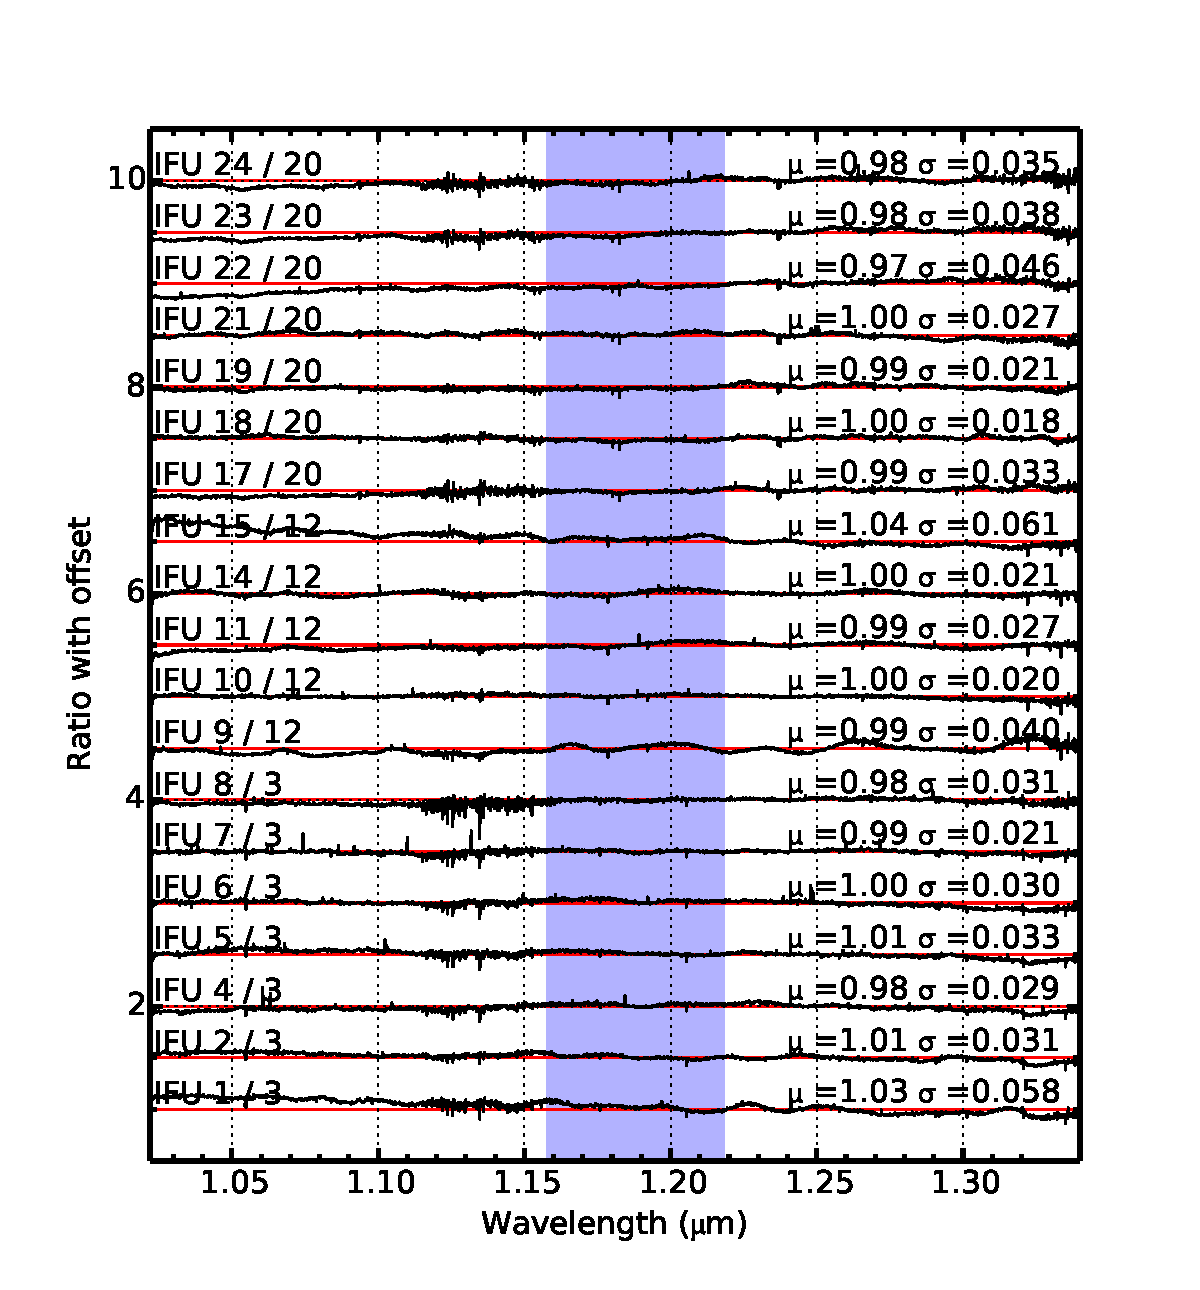
\includegraphics[width=12.0cm]{ngc6822/N6822_t_compare}
 \caption[Comparison of uniformity IFU spectra]{
    Comparison of $J$-band spectra of the same standard star in each IFU.
    The ratio of each spectrum compared to that from the IFU used in the three-arm telluric method is shown,
    with their respective mean and standard deviation ($\mu$ and $\sigma$).
    Red lines indicate $\mu$~=~1.0, $\sigma$~=~0.0 for each ratio.
    The blue shaded area signifies the region used in our analysis,
    within which, the discrepancies between the IFUs are generally small.
    This is reflected in the standard deviation values when only considering this region.
    (IFUs 13 and 16 are omitted as no data were taken with these IFUs.) \label{fig:IFU_compare}
          }
 \end{center}
\end{figure*}

To quantify the difference the two telluric methods would make to our analysis,
we performed the steps described in
Section~\ref{sub:ngc6822_telluric_correction} for both templates.
We then used the two sets of reduced science data
(reduced with both methods of the telluric correction) to compute stellar parameters for our targets.
The results of this comparison are detailed in Section
\ref{sub:telluric_comparison}.

% subsection three_arm_vs_24_arm_telluric_correction (end)

\subsection{Telluric Correction Implementation} % (fold)
\label{sub:ngc6822_telluric_correction}

To improve the accuracy of the telluric correction,
for both methods mentioned above,
we implemented additional recipes beyond those of the KMOS/esorex pipeline.
These recipes were employed to account for two effects which could potentially degrade the quality of the telluric correction.
The first corrects for any potential shift in wavelength between each science spectrum and its associated telluric standard.
The most effective way to implement this is to cross-correlate each pair of science and telluric-standard spectra.
Any shift between the two is then applied to the telluric standard using a cubic-spline interpolation routine.

The second correction applied is a simple spectral scaling algorithm.
This routine corrects for differences in line intensity of the most prominent features common to both the telluric and science spectra.
To find the optimal scaling parameter the following formula is used,

\begin{equation} \label{eq:shiftandres}
T_{2} = (T_{1} + c) / (1 + c),
\end{equation}

\noindent where $T_{2}$ is the corrected telluric-standard spectrum,
$T_{1}$ is the initial telluric standard spectrum and $c$ is the scaling parameter.

To determine the required scaling,
telluric spectra are computed for $-0.5<c<0.5$, in increments of 0.02
(where a perfect value, i.e. no difference in line strength, would be $c$~=~0).
Each telluric spectrum is used to correct the science data and the standard deviation of the counts across the spectral region is computed for each corrected spectrum.
The minimum value of the standard-deviation matrix defines the optimum scaling.
For this algorithm, only the region of interest for our analysis is considered
(i.e. 1.16-1.22\,$\mu$m).

The final set of telluric-standard spectra from the KMOS/esorex reductions were modified using these additional routines and were then used to correct the science observations for the effects of the Earth's atmosphere.



\begin{figure*}
 \centering
 %\vspace{302pt}
 \begin{center}
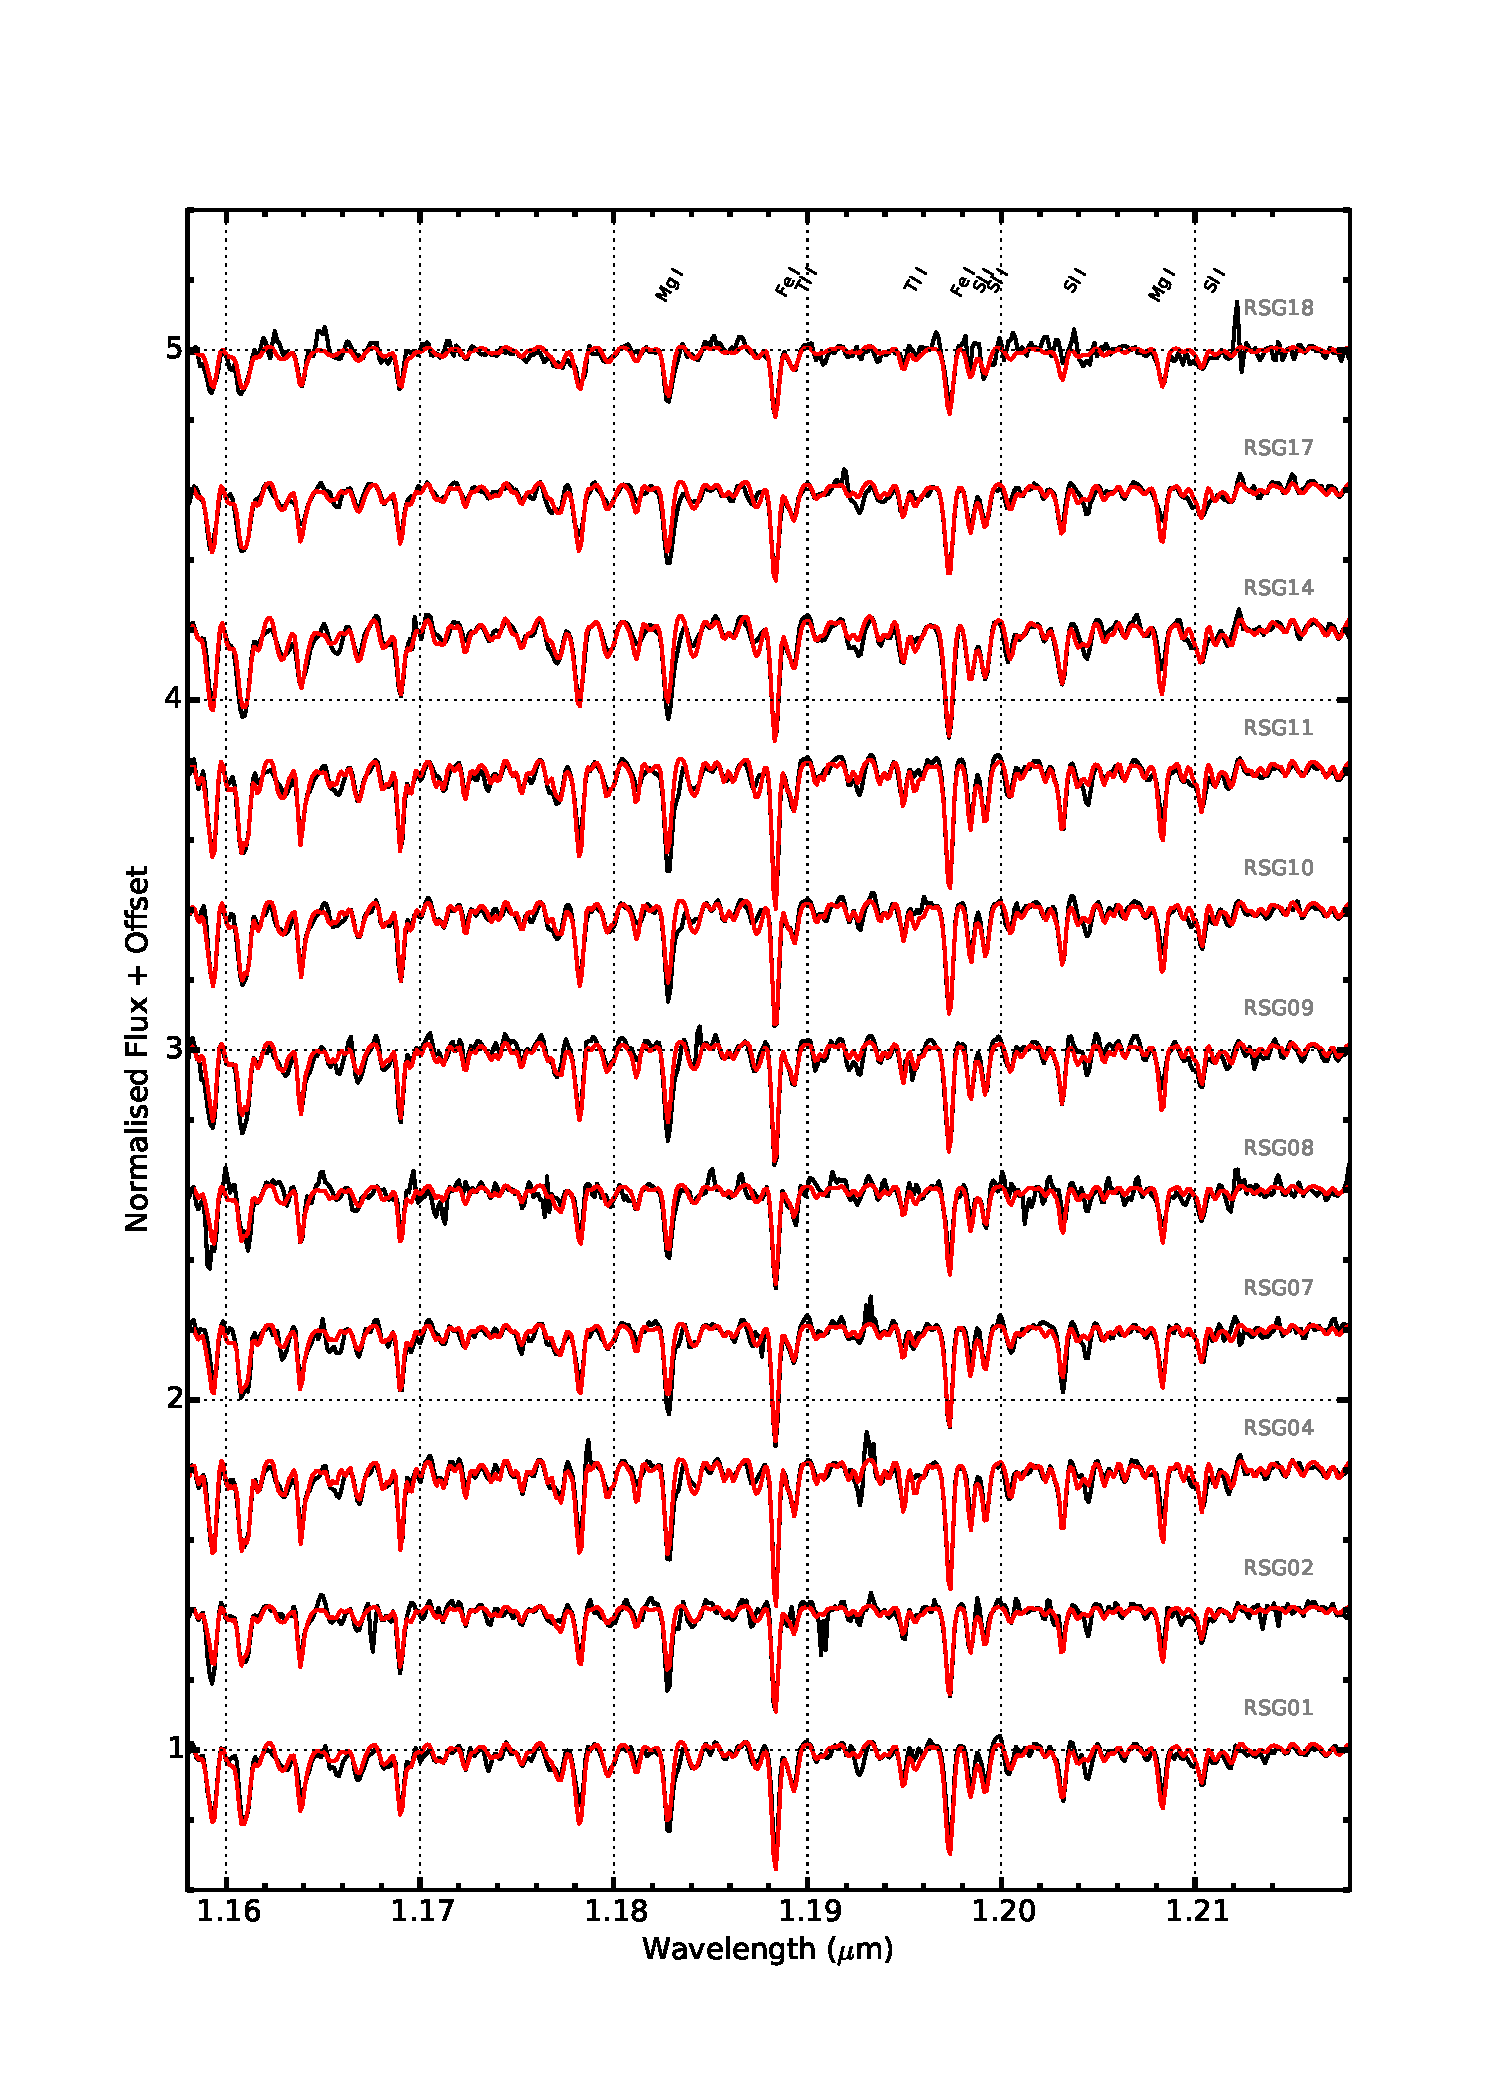
\includegraphics[width=\textwidth]{ngc6822/N6822_mod_fit.pdf}
\caption[Observed and best-fit model spectra]{
KMOS spectra of the NGC\,6822 RSGs and their associated best-fit model spectra
(black and red lines, respectively).
The lines used for the analysis from left-to-right by species are:
Fe\,\1$\lambda\lambda$1.188285,
1.197305,
Si\,\1$\lambda\lambda$1.198419,
1.199157,
1.203151,
1.210353,
Ti\,\1$\lambda\lambda$1.189289,
1.194954.
The two strong Mg\,\1 lines are also labelled, but are not used in the fits
(see Section~\ref{sec:results}).
         }
\label{fig:model_fits}
\end{center}
\end{figure*}


\begin{table*}
\scriptsize
 \caption[$c$-values]{
    Cross-correlation shift values and rescaling ($c$) values.
    }
 \label{c value}
 \begin{center}
  \begin{tabular}{lccccc}
   \hline
 Name  & \multicolumn{2}{c}{24 AT}  & \multicolumn{2}{c}{3 AT} \\
 &  Shift &  $c$  & Shift &  $c$\\
   \hline
   NGC6822-RSG01 &  0.143 & 0.112  &  0.051 & 0.130  \\ % N6822\_5  & J194443.81-144610.7
   NGC6822-RSG02 &  0.135 & 0.140  &  0.184 & 0.216  \\ % N6822\_8  & J194445.98-145102.4
   NGC6822-RSG03 &  0.115 & 0.104  &  0.036 & 0.112  \\ % N6822\_9  & J194447.13-144627.1
   NGC6822-RSG04 &  0.133 & 0.122  &  0.133 & 0.122  \\ % N6822\_12 & J194447.81-145052.5
   NGC6822-RSG05 &  0.054 & 0.198  & -0.017 & 0.206  \\ % N6822\_16 & J194450.54-144801.6
   NGC6822-RSG06 &  0.127 & 0.224  &  0.163 & 0.226  \\ % N6822\_21 & J194451.64-144858.0
   NGC6822-RSG07 & -0.048 & 0.148  &  0.052 & 0.092  \\ % N6822\_24 & J194453.46-144552.6
   NGC6822-RSG08 &  0.062 & 0.180  &  0.062 & 0.180  \\ % N6822\_25 & J194453.46-144540.1
   NGC6822-RSG09 &  0.077 & 0.060  &  0.012 & 0.090  \\ % N6822\_29 & J194454.46-144806.2
   NGC6822-RSG10 & -0.014 & 0.102  &  0.150 & 0.134  \\ % N6822\_30 & J194454.54-145127.1
   NGC6822-RSG11 &  0.067 & 0.134  &  0.060 & 0.110  \\ % N6822\_34 & J194455.70-145155.4
   NGC6822-RSG12 &  0.007 & 0.228  & -0.019 & 0.182  \\ % N6822\_36 & J194455.93-144719.6
   NGC6822-RSG13 & -0.329 & 0.290  & -0.310 & 0.342  \\ % N6822\_39 & J194456.86-144858.5
   NGC6822-RSG14 & -0.464 & 0.138  & -0.021 & 0.258  \\ % N6822\_40 & J194457.31-144920.2
   NGC6822-RSG15 & -0.324 & 0.206  & -0.585 & 0.250  \\ % N6822\_45 & J194459.14-144723.9
   NGC6822-RSG16 & -0.230 & 0.196  & -0.207 & 0.244  \\ % N6822\_47 & J194500.24-144758.9
   NGC6822-RSG17 & -0.192 & 0.160  & -0.192 & 0.160  \\ % N6822\_49 & J194500.53-144826.5
   NGC6822-RSG18 & -0.521 & 0.366  & -0.458 & 0.364  \\ % N6822\_55 & J194506.98-145031.1
   \hline
  \end{tabular}
 \end{center}
\end{table*}


% subsection ngc6822_telluric_correction (end)

\subsection{MOLECFIT} % (fold)
\label{sub:molecfit}

As an alternative to observing telluric standard stars, a new telluric correction package, {\sc molecfit}, allows one to calculate a telluric spectrum based on atmospheric modelling.
Briefly, the software uses a reference atmospheric profile to estimate the true profile for the time and location of the science observation.
This model is then used to create a telluric spectrum which can be used to correct the observations.

This software has been shown to work well, on a variety of VLT instruments
\citep{2015A&A...576A..77S} and has been rigorously tested using X-shooter spectra
\citep{2015A&A...576A..78K}.
However, the package has yet to be tested thoroughly on lower-resolution observations such as those from KMOS.
Our first tests appear encouraging, however, pending further characterisation of the KMOS data cubes
(e.g., small variations in spectral resolving power leading to sky residuals,
see Section~\ref{sub:sky_subtraction}),
I will investigate the potential of the {\sc molecfit} package with KMOS in the future.
% subsection molecfit (end)


\subsection{Stellar Radial Velocities} % (fold)
\label{sub:RVs}


Radial velocities for each target are listed in Table~\ref{tb:obs-params}.
The method used here to measure radial velocity values is consistent with that presented in \textbf{Chapter x.xx (i.e. as NGC\,2100)}.
Briefly, radial velocities are calculated using an iterative cross-correlation method.
Initially, the accuracy of the wavelength solution provided by the data reduction pipeline is checked against a spectrum of the Earth's telluric features.
Any offset is accounted for and the science spectrum is now assumed to be at ``rest'' wavelength.

Once the science spectra are at ``rest'' wavelength, the spectra are then cross-correlated again an appropriate synthetic RSG model using a large region where stellar features are known to dominate ($1.16-1.22\mu$m).
This initial guess is then improved on by selecting seven of the strongest spectral lines in this region and a radial velocity is calculated for each of these lines.
The final radial velocity is the mean of these seven strong lines where the error on the measurement is the standard deviation of the measurements normalised by the number of measurements
($err$~=~$\sigma_{rv}/N$).


Radial velocities estimates are shown as a function of distance to the centre of NGC\,6822 in Figure~\ref{fig:RvsRV}.
The average radial velocity for our targets is $-62\pm13$\,\kms,
in good agreement with the systemic radial velocity of the H\,\1 disk
\citep[$-57\pm2$\,\kms;][]{2004AJ....128...16K}.
Our radial velocities also agree with estimates for the two A-type supergiants from
\cite{2001ApJ...547..765V}.
This result confirms that our candidates are NGC\,6822 members.

\begin{figure}
 \centering
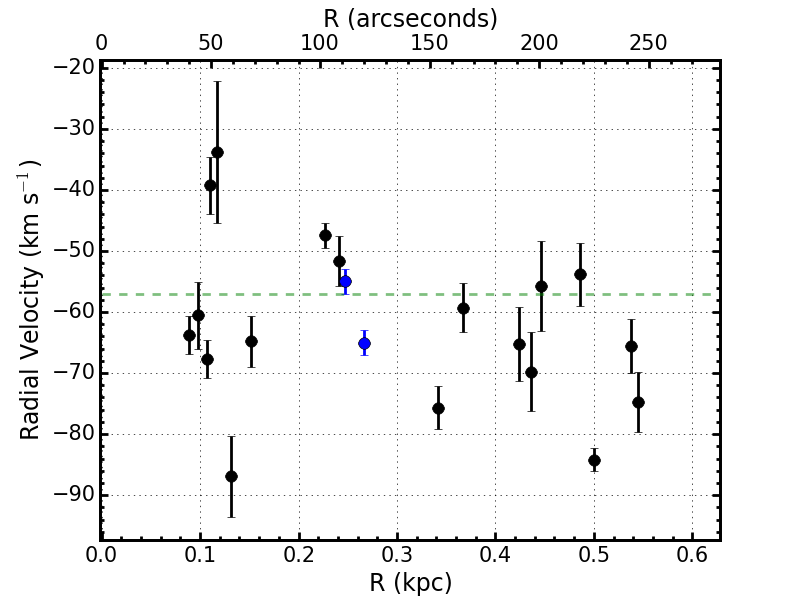
\includegraphics[width=0.65\textwidth]{ngc6822/N6822_RvsRV-v2}
\caption[Radial velocities shown against distance from galaxy centre]{
Radial velocities of targets shown against their distance from the galaxy centre.
The average radial velocity for the sample is $-62\pm13$\,\kms.
The green dashed line indicates H\,\1 systemic velocity
\protect\citep[$-57\pm2$\,\kms;][]{2004AJ....128...16K}.
The radial velocities of two A-type supergiants from
\protect\cite{2001ApJ...547..765V} are shown in blue.
        }
\label{fig:RvsRV}
\end{figure}

% subsection RVs (end)
% section data_reduction_and_analysis (end)


\section{Results} % (fold)
\label{sec:results}

Stellar parameters
(metallicity, effective temperature, surface gravity and microturbulence)
have been derived using the $J$-band analysis technique described by
\cite{2010MNRAS.407.1203D} and demonstrated by
\cite{2014ApJ...788...58G} and
\cite{2015ApJ...806...21D}.
To estimate physical parameters this technique uses a grid of synthetic spectra to fit observational data,
in which the models are degraded to the resolution of the observed spectra
(Table~\ref{tb:res}).
Model atmospheres were generated using the {\sc marcs} code
{\citep{2008A&A...486..951G}} where the range of parameters are defined in
Table~\ref{tb:mod_range}.
The precision of the models is increased by including departures from LTE in some of the strongest Fe, Ti and Si atomic lines
\citep{2012ApJ...751..156B,2013ApJ...764..115B}.
The two strong magnesium lines in our diagnostic spectral region are initially excluded from the analysis as these lines are known to be affected strongly by non-LTE effects
(see Figure~\ref{fig:model_fits}, where the two Mg\,\1 lines are systematically under- and over-estimated, respectively).
This is discussed further in Section~\ref{sub:with_mg}.


\begin{table}
\caption{
Model grid used for analysis.\label{tb:mod_range}
         }
\scriptsize
\begin{center}
\begin{tabular}{lccc}
 \hline
 \hline
  Model Parameter & Min. & Max. & Step size \\
 \hline
T$_{eff}$ (K)        & 3400 & 4000 & 100 \\
                     & 4000 & 4400 & 200 \\
$[$Z$]$ (dex)   & $-$1.50 & 1.00  & 0.25\\
log\,$g$ (cgs)  & $-$1.0\o & 1.0\o & 0.5\o \\
 $\xi$ (\kms)  & \pp1.0\o & 6.0\o & 1.0\o\\
 \hline
\end{tabular}
\end{center}
\end{table}

% subsection telluric_comparison (end)

\subsection{Telluric Comparison} % (fold)
\label{sub:telluric_comparison}

We used these Science Verification data to determine which of the two telluric standard methods is most appropriate for our analysis.
Table~\ref{tb:stellar-params} details the stellar parameters estimated for each target using both telluric methods and these parameters are compared in
Figure~\ref{fig:3vs24AT}.
The mean difference in the parameters between the two methods is
$<\Delta \xi>$~=~$-0.1 \pm 0.1$,
$\Delta [$Z$]$~=~$0.04\pm 0.07$,
$<\Delta$ log\,$g>$~=~$-0.06 \pm 0.12$ and
$<\Delta $T$_{\rm eff}>$~=~$-14 \pm 42$.
Therefore, for our analysis, there appears to be no significant difference between the two telluric approaches.


\begin{figure*}
 \centering
 \begin{center}$
  \centering
  \begin{array}{cc}
  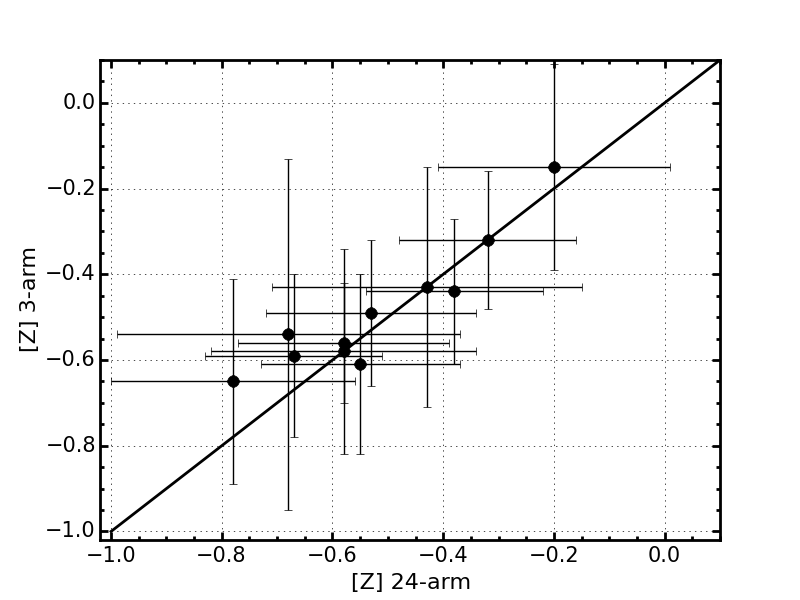
\includegraphics[width=0.5\textwidth]{ngc6822/N6822_24vs3AT_Z} &
  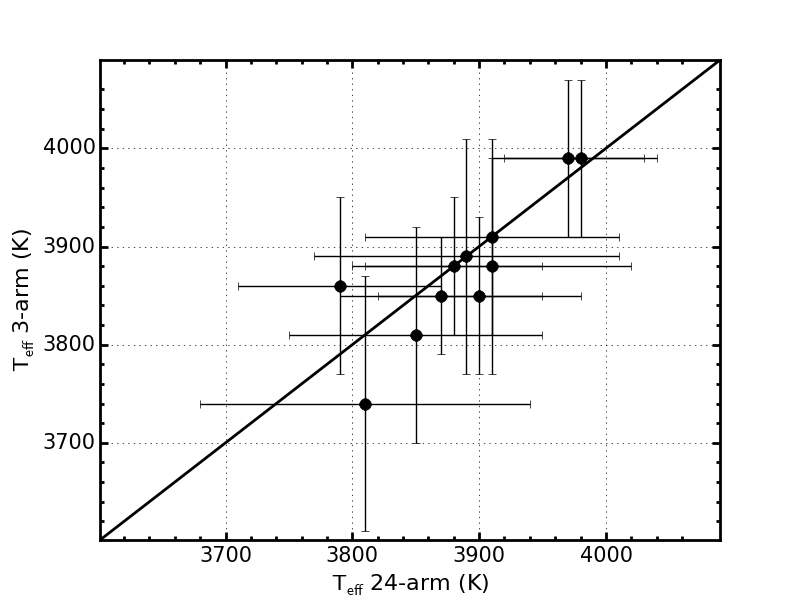
\includegraphics[width=0.5\textwidth]{ngc6822/N6822_24vs3AT_Teff} \\
  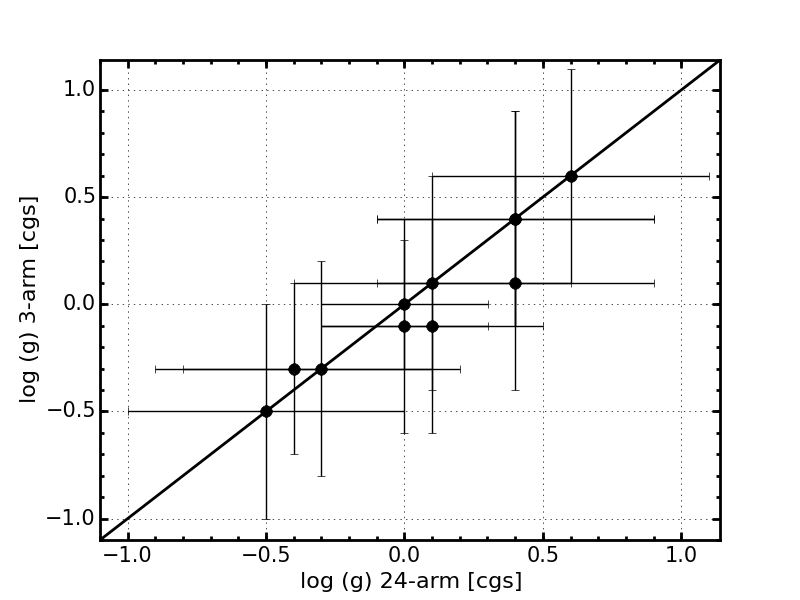
\includegraphics[width=0.5\textwidth]{ngc6822/N6822_24vs3AT_logg} &
  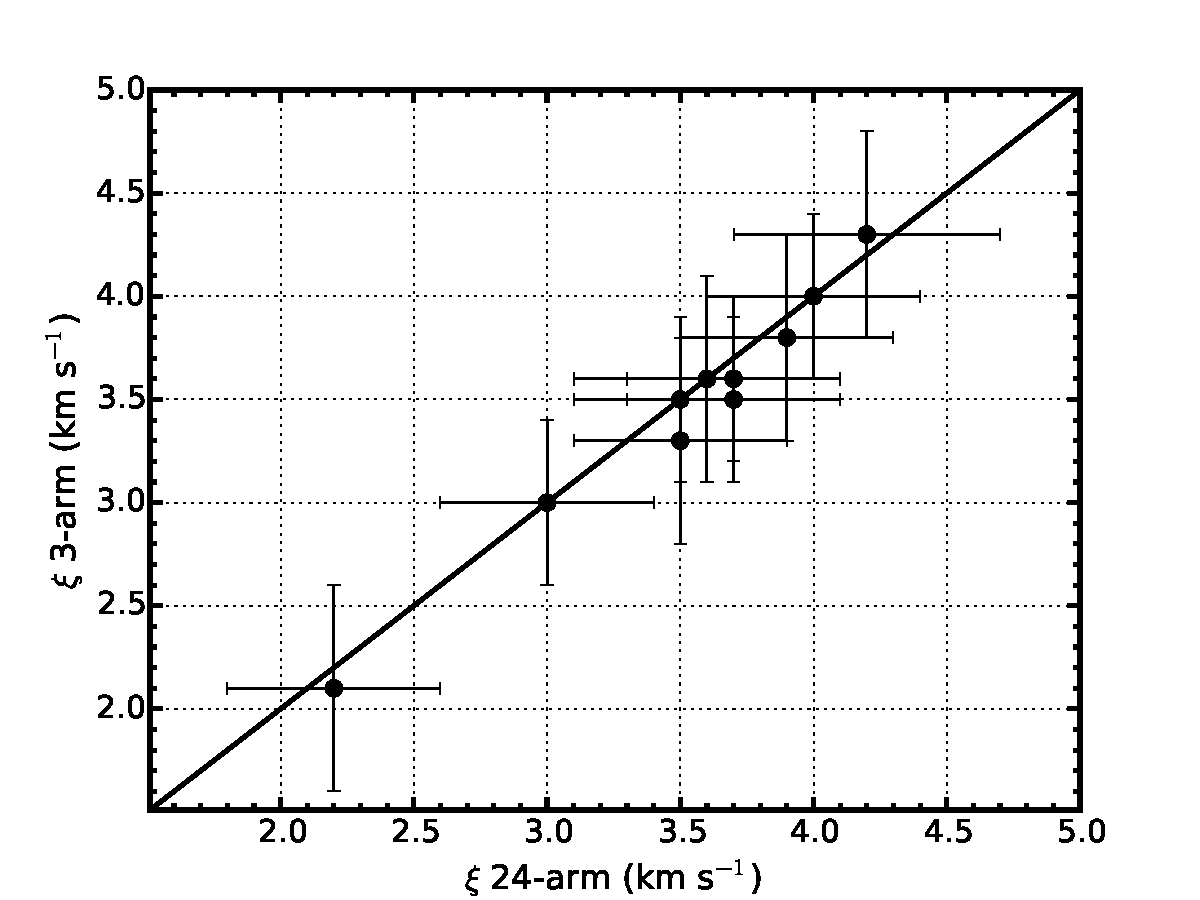
\includegraphics[width=0.5\textwidth]{ngc6822/N6822_24vs3AT_Xi} \\
  \end{array}$
 \end{center}
 \caption[Best-fit parameter comparison using the two telluric methods]{
            Comparison of the model parameters using the two different telluric methods.
            In each panel, the x-axis represents stellar parameters estimated using the 3 arm telluric
            method and the y-axis represents those estimated using the 24 arm telluric method.
            Top left: metallicity ([Z]), mean difference
            $<\Delta[$Z$]>$~=~$0.04 \pm 0.07$.
            Top right: effective temperature (T$_{\rm eff}$), mean difference
            $<\Delta $T$_{\rm eff}>$~=~$-14 \pm 42$.
            Bottom left: surface gravity (log\,$g$), mean difference
            $<\Delta$ log\,$g>$~=~$-0.06 \pm 0.12$.
            Bottom right: Microturbulence ($\xi$), mean difference
            $<\Delta \xi>$~=~$-0.1 \pm 0.1$.
            % Green dashed lines indicates linear best fits to the data.
            In all cases, the distributions are statistically consistent with a one-to-one ratio (black lines).
          }
 \label{fig:3vs24AT}
\end{figure*}


\begin{sidewaystable}
\begin{center}
\caption{
Fit parameters for reductions using the two different telluric methods.
\label{tb:stellar-params}
         }
\scriptsize
\begin{tabular}{lc cccc c cccc}
 \hline
 \hline
  Target  & IFU &  \multicolumn{4}{c}{24 Arm Telluric} & \multicolumn{4}{c}{3 Arm Telluric}\\
  \cline{3-6}  \cline{8-11}
 &  & T$_{eff}$ (K) & log\,$g$ & $\xi$ (\kms) & [Z] & & T$_{eff}$ (K) & log\,$g$ & $\xi$ (\kms) & [Z]\\
  \hline
NGC6822-RSG01 & 6 & 3790 $\pm$ 80\o & $-$0.0 $\pm$ 0.3 & 3.5 $\pm$ 0.4 & $-$0.55 $\pm$ 0.18 & & 3860 $\pm$ 90\o & $-$0.1 $\pm$ 0.5 &  3.5 $\pm$ 0.4 & $-$0.61 $\pm$ 0.21 \\
NGC6822-RSG02 & 11& 3850 $\pm$ 100  & \pp0.4 $\pm$ 0.5 & 3.5 $\pm$ 0.4 & $-$0.78 $\pm$ 0.22 & & 3810 $\pm$ 110  & \pp0.4 $\pm$ 0.5 &  3.3 $\pm$ 0.5 & $-$0.65 $\pm$ 0.24 \\
NGC6822-RSG04 & 12& 3880 $\pm$ 70\o & \pp0.0 $\pm$ 0.3 & 4.0 $\pm$ 0.4 & $-$0.32 $\pm$ 0.16 & & 3880 $\pm$ 70\o & \pp0.0 $\pm$ 0.3 &  4.0 $\pm$ 0.4 & $-$0.32 $\pm$ 0.16 \\
NGC6822-RSG07 & 2 & 3970 $\pm$ 60\o & \pp0.4 $\pm$ 0.5 & 3.9 $\pm$ 0.4 & $-$0.58 $\pm$ 0.19 & & 3990 $\pm$ 80\o & \pp0.1 $\pm$ 0.5 &  3.8 $\pm$ 0.5 & $-$0.56 $\pm$ 0.14 \\
NGC6822-RSG08 & 3 & 3910 $\pm$ 100  & \pp0.6 $\pm$ 0.5 & 3.0 $\pm$ 0.4 & $-$0.58 $\pm$ 0.24 & & 3910 $\pm$ 100  & \pp0.6 $\pm$ 0.5 &  3.0 $\pm$ 0.4 & $-$0.58 $\pm$ 0.24 \\
NGC6822-RSG09 & 4 & 3980 $\pm$ 60\o & \pp0.1 $\pm$ 0.4 & 3.7 $\pm$ 0.4 & $-$0.38 $\pm$ 0.16 & & 3990 $\pm$ 80\o & $-$0.1 $\pm$ 0.5 &  3.6 $\pm$ 0.4 & $-$0.44 $\pm$ 0.17 \\
NGC6822-RSG10 & 14& 3900 $\pm$ 80\o & $-$0.3 $\pm$ 0.5 & 3.7 $\pm$ 0.4 & $-$0.67 $\pm$ 0.16 & & 3850 $\pm$ 80\o & $-$0.3 $\pm$ 0.5 &  3.5 $\pm$ 0.4 & $-$0.59 $\pm$ 0.19 \\
NGC6822-RSG11 & 15& 3870 $\pm$ 80\o & $-$0.4 $\pm$ 0.5 & 4.2 $\pm$ 0.5 & $-$0.53 $\pm$ 0.19 & & 3850 $\pm$ 60\o & $-$0.3 $\pm$ 0.4 &  4.3 $\pm$ 0.5 & $-$0.49 $\pm$ 0.17 \\
NGC6822-RSG14 & 17& 3910 $\pm$ 110  & $-$0.5 $\pm$ 0.5 & 3.6 $\pm$ 0.5 & $-$0.20 $\pm$ 0.21 & & 3880 $\pm$ 110  & $-$0.5 $\pm$ 0.5 &  3.6 $\pm$ 0.5 & $-$0.15 $\pm$ 0.24 \\
NGC6822-RSG17 & 21& 3890 $\pm$ 120  & \pp0.1 $\pm$ 0.5 & 3.0 $\pm$ 0.4 & $-$0.43 $\pm$ 0.28 & & 3890 $\pm$ 120  & \pp0.1 $\pm$ 0.5 &  3.0 $\pm$ 0.4 & $-$0.43 $\pm$ 0.28 \\
NGC6822-RSG18 & 18& 3810 $\pm$ 130  & \pp0.4 $\pm$ 0.5 & 2.2 $\pm$ 0.4 & $-$0.68 $\pm$ 0.31 & & 3740 $\pm$ 130  & \pp0.4 $\pm$ 0.5 &  2.1 $\pm$ 0.5 & $-$0.54 $\pm$ 0.41 \\

% Stars not included in the sample:

% RSG9  & 5 & 4040 $\pm$ 130  & \pp0.8 $\pm$ 0.3 & 3.8 $\pm$ 0.6 & \pp0.14 $\pm$ 0.24 & 2500 & & 3990 $\pm$ 130  & \pp0.8 $\pm$ 0.3 &  3.8 $\pm$ 0.6 & \pp0.09 $\pm$ 0.24 & 2500 \\
% RSG16 & 7 & 4200 $\pm$ 50\o & \pp0.5 $\pm$ 0.4 & 2.3 $\pm$ 0.3 & $-$0.51 $\pm$ 0.16 & 4400 & & 4230 $\pm$ 100  & \pp0.5 $\pm$ 0.2 &  2.4 $\pm$ 0.3 & $-$0.54 $\pm$ 0.15 & 4400 \\
% RSG21 & 10& 3780 $\pm$ 110  & \pp0.4 $\pm$ 0.5 & 2.3 $\pm$ 0.4 & $-$0.55 $\pm$ 0.32 & 3800 & & 3790 $\pm$ 90\o & \pp0.5 $\pm$ 0.5 &  2.2 $\pm$ 0.4 & $-$0.46 $\pm$ 0.33 & 3800 \\
% RSG36 & 1 & 3840 $\pm$ 120  & \pp0.6 $\pm$ 0.5 & 3.0 $\pm$ 0.4 & $-$0.52 $\pm$ 0.26 & 3300 & & 3930 $\pm$ 100  & \pp0.6 $\pm$ 0.4 &  2.9 $\pm$ 0.4 & $-$0.39 $\pm$ 0.25 & 3300 \\
% RSG39 & 19& 3870 $\pm$ 130  & \pp0.5 $\pm$ 0.5 & 2.4 $\pm$ 0.5 & $-$0.73 $\pm$ 0.26 & 3000 & & 3800 $\pm$ 120  & \pp0.4 $\pm$ 0.5 &  2.1 $\pm$ 0.5 & $-$0.58 $\pm$ 0.33 & 3000 \\
% RSG45 & 24& 4220 $\pm$ 120  & \pp0.6 $\pm$ 0.5 & 2.9 $\pm$ 0.4 & $-$0.24 $\pm$ 0.20 & 3200 & & 4290 $\pm$ 120  & \pp0.6 $\pm$ 0.5 &  3.0 $\pm$ 0.5 & $-$0.27 $\pm$ 0.22 & 3200 \\
% RSG47 & 22& 3980 $\pm$ 90\o & \pp0.4 $\pm$ 0.4 & 3.2 $\pm$ 0.4 & $-$0.57 $\pm$ 0.23 & 2700 & & 3950 $\pm$ 100  & \pp0.4 $\pm$ 0.4 &  3.3 $\pm$ 0.4 & $-$0.64 $\pm$ 0.24 & 2700 \\

  \hline
  \end{tabular}
  \end{center}
\end{sidewaystable}

\subsection{The Introduction of Magnesium} % (fold)
\label{sub:with_mg}

Since the publication of~\citet[][where the results from this chapter are published]{2015ApJ...803...14P}, non-LTE corrections have been calculated by~\cite{2015ApJ...804..113B}.
Using these results, the model grids have now been updated to include the corrections for non-LTE for the Mg\,\1 lines.
As an additional calibration to these corrections~\citep[to the extensive testing in][]{2015ApJ...804..113B} I have used the updated model grids to re-analyse the NGC\,6822 KMOS spectra.
This allows a direct comparison between results including and excluding the Mg\,\1 lines.


% By implementing these corrections to the model grid stellar parameters can now be calculated including the Mg\,\1 lines.

Figure~\ref{fig:24ATvs24Mg} displays the stellar parameters estimated including and excluding the two Mg\,\1 lines.
This figure shows that there exists no significant difference between the results when the Mg\,\1 lines are included.
Table~\ref{tb:stellar-params-Mg} details the parameters.

For the remainder of this chapter we adopt the updated stellar parameters including the non-LTE effects of Magnesium.

\begin{figure*}
 \centering
 \begin{center}
  \centering
  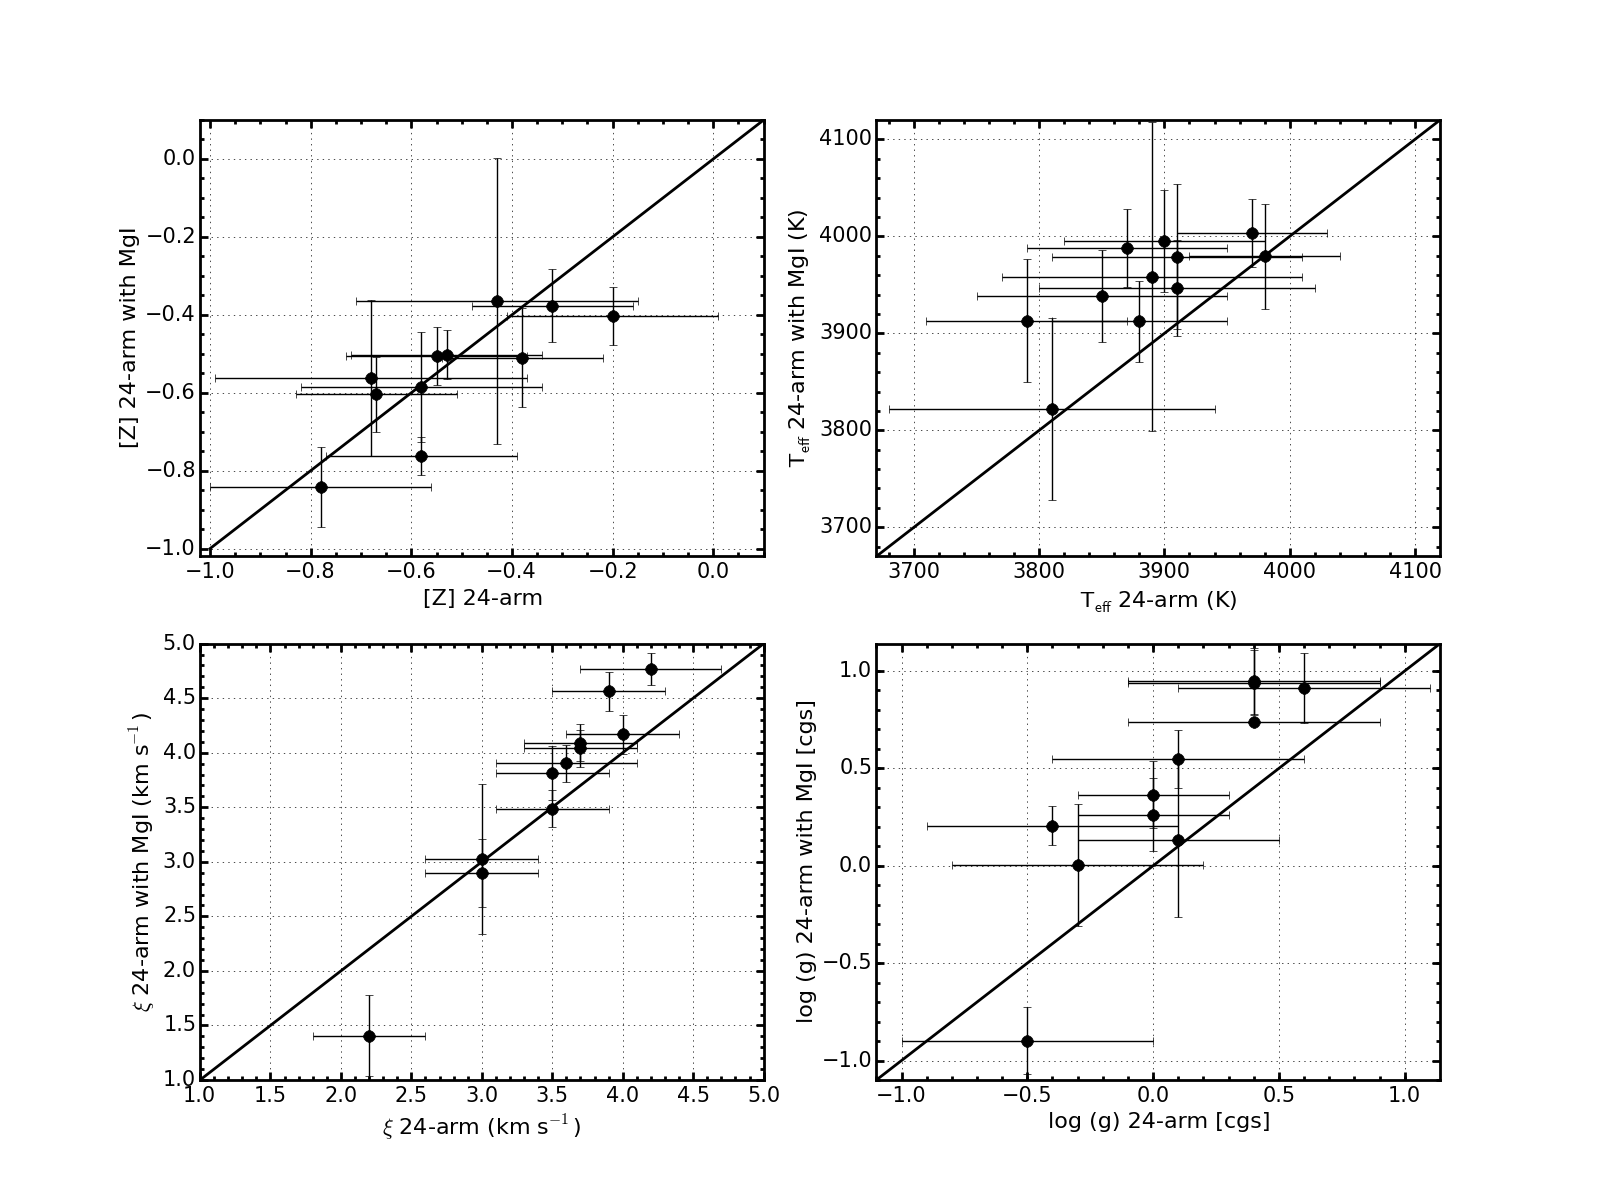
\includegraphics[width=\textwidth]{ngc6822/N6822-Mg-compare}
 \end{center}
 \caption[Best-fit parameter comparison using including and excluding Mg\,\1]{
            Comparison of the model parameters including and excluding Mg\,\1 lines.
            In each panel, the x-axis represents stellar parameters estimated excluding the Mg\,\1 lines
            and the y-axis represents those estimated including the Mg\,\1 lines.
            Top left: metallicity ([Z]), mean difference
            $<\Delta[$Z$]>$~=~0.03$\pm$0.10.
            Top right: effective temperature (T$_{\rm eff}$), mean difference
            $<\Delta$T$_{\rm eff}>$~=~$-$61$\pm$39.
            Bottom left: surface gravity (log\,$g$), mean difference
            $<\Delta$log\,$g>$~=~$-$0.11$\pm$0.37.
            Bottom right: Microturbulence ($\xi$), mean difference
            $<\Delta \xi>$~=~$-$0.17$\pm$0.38.
            % Green dashed lines indicates linear best fits to the data.
            In all cases, the distributions are statistically consistent with a one-to-one ratio (black lines).
          }
 \label{fig:24ATvs24Mg}
\end{figure*}


\begin{sidewaystable}
\begin{center}
\caption{
Fit parameters including and excluding Mg\,\1 lines.
\label{tb:stellar-params-Mg}
         }
\scriptsize
\begin{tabular}{lc cccc c cccc}
 \hline
 \hline
  Target  & IFU &  \multicolumn{4}{c}{24 Arm Telluric without Mg\,I} & \multicolumn{4}{c}{24 Arm Telluric with Mg\,\1}\\
  \cline{3-6}  \cline{8-11}
 &  & $\xi$ (\kms) & [Z] & log\,$g$ & T$_{eff}$ (K) & & $\xi$ (\kms) & [Z] & log\,$g$ & T$_{eff}$ (K)\\
  \hline
NGC6822-RSG01 & 6 & 3.5$\pm$0.4 & $-$0.55$\pm$0.18 & $-$0.0$\pm$0.3 & 3790$\pm$80\o & & 3.5$\pm$0.2 & $-$0.51$\pm$0.07 & \pp0.26$\pm$0.19 & 3910$\pm$60\o\\
NGC6822-RSG02 & 11& 3.5$\pm$0.4 & $-$0.78$\pm$0.22 & \pp0.4$\pm$0.5 & 3850$\pm$100  & & 3.8$\pm$0.2 & $-$0.84$\pm$0.10 & \pp0.94$\pm$0.17 & 3940$\pm$50\o\\
NGC6822-RSG04 & 12& 4.0$\pm$0.4 & $-$0.32$\pm$0.16 & \pp0.0$\pm$0.3 & 3880$\pm$70\o & & 4.2$\pm$0.2 & $-$0.38$\pm$0.09 & \pp0.36$\pm$0.17 & 3910$\pm$40\o\\
NGC6822-RSG07 & 2 & 3.9$\pm$0.4 & $-$0.58$\pm$0.19 & \pp0.4$\pm$0.5 & 3970$\pm$60\o & & 4.6$\pm$0.2 & $-$0.76$\pm$0.05 & \pp0.74$\pm$0.00 & 4000$\pm$40\o\\
NGC6822-RSG08 & 3 & 3.0$\pm$0.4 & $-$0.58$\pm$0.24 & \pp0.6$\pm$0.5 & 3910$\pm$100  & & 2.9$\pm$0.3 & $-$0.59$\pm$0.14 & \pp0.91$\pm$0.18 & 3980$\pm$80\o\\
NGC6822-RSG09 & 4 & 3.7$\pm$0.4 & $-$0.38$\pm$0.16 & \pp0.1$\pm$0.4 & 3980$\pm$60\o & & 4.1$\pm$0.2 & $-$0.51$\pm$0.13 & \pp0.13$\pm$0.40 & 3980$\pm$50\o\\
NGC6822-RSG10 & 14& 3.7$\pm$0.4 & $-$0.67$\pm$0.16 & $-$0.3$\pm$0.5 & 3900$\pm$80\o & & 4.0$\pm$0.2 & $-$0.60$\pm$0.10 & \pp0.00$\pm$0.31 & 4000$\pm$50\o\\
NGC6822-RSG11 & 15& 4.2$\pm$0.5 & $-$0.53$\pm$0.19 & $-$0.4$\pm$0.5 & 3870$\pm$80\o & & 4.8$\pm$0.1 & $-$0.50$\pm$0.06 & \pp0.20$\pm$0.10 & 3990$\pm$40\o\\
NGC6822-RSG14 & 17& 3.6$\pm$0.5 & $-$0.20$\pm$0.21 & $-$0.5$\pm$0.5 & 3910$\pm$110  & & 3.9$\pm$0.2 & $-$0.40$\pm$0.07 & $-$0.90$\pm$0.17 & 3950$\pm$50\o\\
NGC6822-RSG17 & 21& 3.0$\pm$0.4 & $-$0.43$\pm$0.28 & \pp0.1$\pm$0.5 & 3890$\pm$120  & & 3.0$\pm$0.7 & $-$0.36$\pm$0.37 & \pp0.55$\pm$0.15 & 3960$\pm$160\\
NGC6822-RSG18 & 18& 2.2$\pm$0.4 & $-$0.68$\pm$0.31 & \pp0.4$\pm$0.5 & 3810$\pm$130  & & 1.4$\pm$0.4 & $-$0.56$\pm$0.20 & \pp0.95$\pm$0.17 & 3820$\pm$90\o\\

% Stars not included in the sample:

% RSG9  & 5 & 4040 $\pm$ 130  & \pp0.8 $\pm$ 0.3 & 3.8 $\pm$ 0.6 & \pp0.14 $\pm$ 0.24 & 2500 & & 3990 $\pm$ 130  & \pp0.8 $\pm$ 0.3 &  3.8 $\pm$ 0.6 & \pp0.09 $\pm$ 0.24 & 2500 \\
% RSG16 & 7 & 4200 $\pm$ 50\o & \pp0.5 $\pm$ 0.4 & 2.3 $\pm$ 0.3 & $-$0.51 $\pm$ 0.16 & 4400 & & 4230 $\pm$ 100  & \pp0.5 $\pm$ 0.2 &  2.4 $\pm$ 0.3 & $-$0.54 $\pm$ 0.15 & 4400 \\
% RSG21 & 10& 3780 $\pm$ 110  & \pp0.4 $\pm$ 0.5 & 2.3 $\pm$ 0.4 & $-$0.55 $\pm$ 0.32 & 3800 & & 3790 $\pm$ 90\o & \pp0.5 $\pm$ 0.5 &  2.2 $\pm$ 0.4 & $-$0.46 $\pm$ 0.33 & 3800 \\
% RSG36 & 1 & 3840 $\pm$ 120  & \pp0.6 $\pm$ 0.5 & 3.0 $\pm$ 0.4 & $-$0.52 $\pm$ 0.26 & 3300 & & 3930 $\pm$ 100  & \pp0.6 $\pm$ 0.4 &  2.9 $\pm$ 0.4 & $-$0.39 $\pm$ 0.25 & 3300 \\
% RSG39 & 19& 3870 $\pm$ 130  & \pp0.5 $\pm$ 0.5 & 2.4 $\pm$ 0.5 & $-$0.73 $\pm$ 0.26 & 3000 & & 3800 $\pm$ 120  & \pp0.4 $\pm$ 0.5 &  2.1 $\pm$ 0.5 & $-$0.58 $\pm$ 0.33 & 3000 \\
% RSG45 & 24& 4220 $\pm$ 120  & \pp0.6 $\pm$ 0.5 & 2.9 $\pm$ 0.4 & $-$0.24 $\pm$ 0.20 & 3200 & & 4290 $\pm$ 120  & \pp0.6 $\pm$ 0.5 &  3.0 $\pm$ 0.5 & $-$0.27 $\pm$ 0.22 & 3200 \\
% RSG47 & 22& 3980 $\pm$ 90\o & \pp0.4 $\pm$ 0.4 & 3.2 $\pm$ 0.4 & $-$0.57 $\pm$ 0.23 & 2700 & & 3950 $\pm$ 100  & \pp0.4 $\pm$ 0.4 &  3.3 $\pm$ 0.4 & $-$0.64 $\pm$ 0.24 & 2700 \\

  \hline
  \end{tabular}
  \end{center}
\end{sidewaystable}


% subsection the_introduction_of_magnesium (end)

\subsection{Stellar Parameters and Metallicity} % (fold)
\label{sub:stellar_parameters_and_metallicity}

Table~\ref{tb:stellar-params-Mg} summarises the estimated stellar parameters.
For the remainder of this chapter, when discussing stellar parameters,
we adopt those estimated using the 24 arm telluric method including the Mg\,\1 lines.
(i.e. the results in the left-hand part of Table~\ref{tb:stellar-params-Mg}.)
The average metallicity for our sample of 11 RSGs in NGC\,6822 is
$\bar{Z}$~=~$-0.55\pm0.13$.
This result is in good agreement with the average metallicity estimated in
\citet[][see also Figure~\ref{fig:ZvsR}]{2015ApJ...803...14P}.
In addition the results presented here are also in good agreement with results using BSGs
\citep[BSGs;][]{1999A&A...352L..40M,2001ApJ...547..765V}.

A direct comparison with metallicities from BSGs is legitimate as the method used in the present analysis yield a global metallicity ([Z]) which
closely resembles the Fe/H ratio estimated in
\cite{2001ApJ...547..765V}.
While our [Z] measurements are also affected by Si and Ti,
we assume [Z]~=~[Fe/H] for the purposes of our discussion.
Likewise, we can compare oxygen abundances (relative to solar) obtained from H\,\2 regions as a proxy for [Z] by
introducing the solar oxygen abundance
{12+log\,(O/H)}$_{\odot}$~=~8.69
\citep{2009ARA&A..47..481A} through the relation
[Z]~=~$12 + $log\,(O/H)$ - 8.69$.
This implicitly assumes that the $\alpha$/Fe ratio remains Solar in different environments.

As outlined in \textbf{Chapter x.x} the RSG and BSG stages are different evolutionary phases within the life cycle of a massive star,
while H\,\2 regions are the birth clouds which give rise to the youngest stellar population.
As the lifetimes of RSGs and BSGs are $<50$Myr,
their metallicity estimates are also expected to be representative of their birth clouds.

To investigate the spatial distribution of chemical abundances in NGC\,6822,
in Figure~\ref{fig:ZvsR}
we show the metallicities of our RSGs as a function of radial distance from the centre of the galaxy,
as well as the results from
\cite{2001ApJ...547..765V} and the indicative estimates from
\cite{1999A&A...352L..40M}.


A least-squares fit to the results from~\cite{2015ApJ...803...14P} reveals a low-significance abundance gradient within the central 1\,kpc of NGC\,6822 of $-0.5\pm0.4\,dex\,$kpc$^{-1}$.
In addition, the extrapolated central metallicity from the fit (i.e. at R~=~0) of [Z]~=~$-0.30\pm0.15\,dex$ remains consistent with the average metallicity assuming no gradient.
However, using the updated stellar parameters the data appears consistent with no gradient ($-0.12\pm0.19\,dex\,$kpc$^{-1}$) even though statistically this is a poorer fit to the data.


\begin{figure}
 \centering
 \begin{center}$
  \centering
  \begin{array}{cc}
  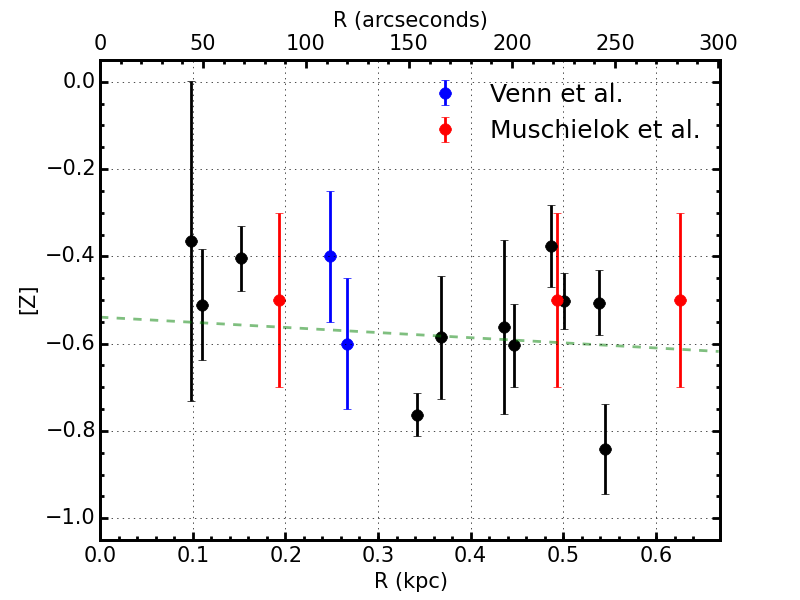
\includegraphics[width=0.5\textwidth]{ngc6822/N6822_ZvsR-thesis} &
  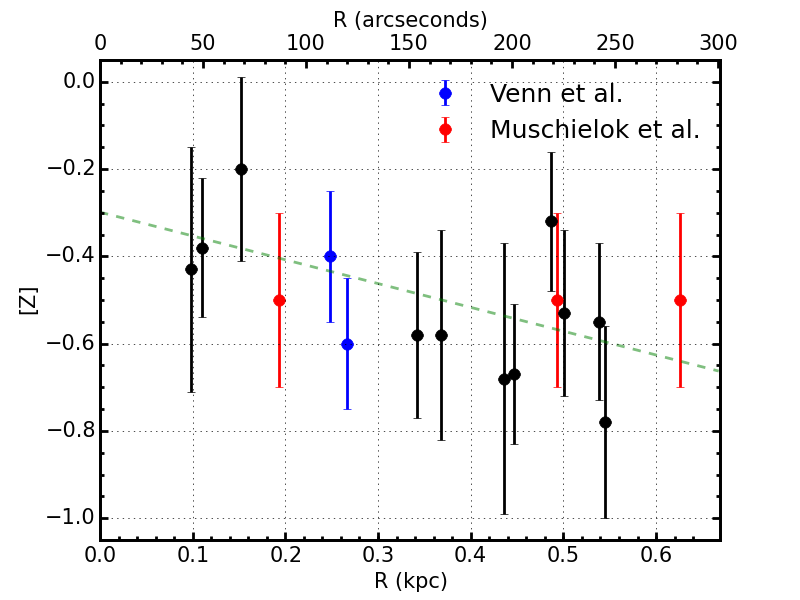
\includegraphics[width=0.5\textwidth]{ngc6822/N6822_ZvsR_BSG} \\
  \end{array}$
 \end{center}
\caption[Metallicities shown against distance from the galaxy centre]{
Estimated metallicities for 11 RSGs in NGC\,6822 shown against their distance from the galaxy centre.
The left panel shows the metallicities estimated including Mg\,\1 lines whereas the right hand panel shows metallicities excluding Mg\,\1.
Blue and red points show BSG results from
\cite{2001ApJ...547..765V} and
\cite{1999A&A...352L..40M} respectively.
The average metallicity is consistent between the two samples and the average including Mg\,\1 is adopted at
$\bar{\rm Z}$~=~$-0.55\pm0.13$.
A least-squares fit to the results excluding Mg\,\1 (right panel) reveals a low-significance abundance gradient
(see text for details).
For comparison,
R$_{25}$~=~460\,arcseconds
\protect\citep[=~1.03\,kpc;][]{2012AJ....144....4M}.
\label{fig:ZvsR}
}
\end{figure}

Figure~\ref{fig:6822HRD} shows the location of our sample in the Hertzsprung-Russell (H-R) diagram.
Bolometric corrections were computed using the calibration in
\cite{2013ApJ...767....3D}.
This figure shows that the temperatures estimated using the $J$-band method are systematically cooler than the end of the evolutionary models (which terminate at the end of the carbon-burning phase for massive stars) for
Z~=~0.002 from
\cite{2013A&A...558A.103G}.
This result is discussed in Section~\ref{sub:temperatures_of_rsgs}.


\begin{figure}
 \centering
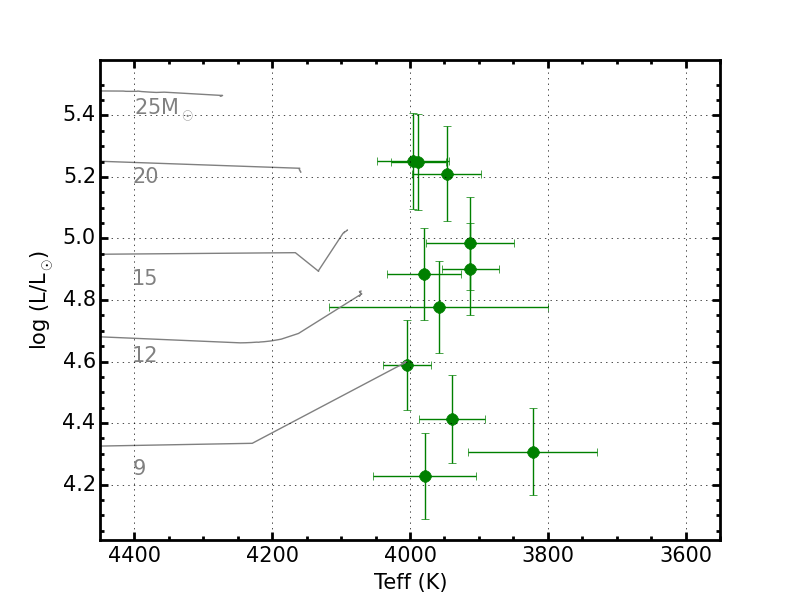
\includegraphics[width=0.65\textwidth]{ngc6822/N6822_HRD_thesis}
\caption[H-R diagram for NGC\,6822]{
H-R diagram for the 11 RSGs in NGC\,6822.
Evolutionary tracks including rotation
($v/v_{c}$~=~0.4) for SMC-like metallicity (Z~=~0.002)
are shown in grey, along with their zero-age mass
\protect\citep{2013A&A...558A.103G}.
Bolometric corrections are computed using the calibration in
\protect\cite{2013ApJ...767....3D}.
We note that compared to the evolutionary tracks,
the observed temperatures of NGC\,6822 RSGs are systematically cooler.
This is discussed in Section~\ref{sub:temperatures_of_rsgs}.
}
\label{fig:6822HRD}
\end{figure}

% subsection stellar_parameters (end)
% section results (end)


\section{Discussion} % (fold)
\label{sec:discussion}

\subsection{Metallicity Measurements} % (fold)
\label{sub:metallicity_measurements}

The average metallicity for the sample is $\bar{\rm Z}$~=~$-$0.55$\pm$0.13,
which agrees well with the results estimated from BSGs
\citep{1999A&A...352L..40M,2001ApJ...547..765V,2002PhDT.........3P} and H\,\2 regions
\citep{2006ApJ...642..813L}.
These results are consistent with no metallicity gradient within NGC\,6822.


Using the data from \citep[][i.e excluding Mg\,\1]{2015ApJ...803...14P} there exists a low-significance metallicity gradient within the central 1\,kpc of NGC\,6822
($-0.5\pm0.4\,dex\,$kpc$^{-1}$ with a $\chi^{2}_{red}$~=~1.16; see Figure~\ref{fig:ZvsR}).
The gradient estimated is consistent with the trend reported in
\cite{2001ApJ...547..765V}
from their results for the two BSGs which these authors compared with H\,\2 regions
\citep{1980MNRAS.193..219P} and two planetary nebulae
\citep{1995ApJ...445..642R} at larger galactocentric distances.
This result is also consistent with the gradient estimated from a sample of 49 local star-forming galaxies
\citep{2015MNRAS.448.2030H}.
Including the results for BSGs from
\cite{2001ApJ...547..765V}
in the analysis,
gives a consistent gradient
($-0.48\pm 0.33\,dex$\,kpc$^{-1}$)
with an improved
$\chi^{2}_{red}$~=~1.06.
Results from
\cite{1999A&A...352L..40M} are not included in the fit as these measurements were qualitative estimates of metallicity.



In contrast,
\cite{2006ApJ...642..813L} used the oxygen abundances from 19 H\,\2
regions and found no clear evidence for a metallicity gradient.
Using a subset of the highest quality H\,\2
region data available, these authors found a gradient of
$-0.16\pm0.05dex\,$kpc$^{-1}$.
Including these results into our analysis degrades the fit and changes the estimated gradient significantly
($-0.18\pm0.05dex\,$kpc$^{-1}$; $\chi^{2}_{red}$~=~1.78).
However, when this data is combined with the RSG data including the Mg\,\1 lines, a significant gradient is measured
($-0.13\pm0.04dex\,$kpc$^{-1}$; $\chi^{2}_{red}$~=~2.91).
At this point it is not clear whether the indication of a gradient obtained from the RSGs and BSGs is an artefact of the small sample size,
or indicates a difference with respect to the H\,\2 region study.


There have been a number of studies of the metallicity of the older stellar population in NGC\,6822.
From spectroscopy of red giant branch (RGB) stars,
\cite{2001MNRAS.327..918T} found a mean metallicity of [Fe/H]~=~$-0.9$
with a reasonably large spread (see their Figure 19).
More recently,
\cite{2012A&A...540A.135S} derived metallicities using a population of AGB stars within the central 4\,kpc of NGC\,6822.
They found an average metallicity of [Fe/H]~=~$-1.29\pm0.07\,dex$.
Likewise,
\cite{2013ApJ...779..102K}
used spectra of red giant stars within the central 2\,kpc and found an average metallicity of
[Fe/H]~=~$-1.05\pm0.49\,dex$.
We note that none of these studies found any compelling evidence for spatial variations in the stellar metallicities,
which is not surprising given that, in disc galaxies, radial migration is thought to smooth out any abundance gradients over time.
The stellar populations used for these studies are known to be significantly older than our sample,
therefore, owing to the chemical evolution in the time since the birth of the older populations,
we expect the measured metallicities to be significantly lower.

The low metallicity of the young stellar population and the interstellar medium (ISM) in NGC\,6822 can be understood as a consequence of the fact that it is a relatively gas-rich galaxy with a mass
M$_{HI}$~=~1.45$\times$10$^{8}$\,M$_{\odot}$
\citep{2004AJ....128...16K} and a total stellar mass of ranging from
M$_{*}$~=~$0.83$~-~$1.70\times$10$^{8}$ M$_{\odot}$
\citep{2008MNRAS.390.1453W,2013ApJ...779..102K,2014ApJ...789..147W}.

The simple closed-box chemical-evolution model relates the metallicity mass fraction $Z(t)$ at any time to the ratio of stellar to gas mass $M_{*}\over M_{g}$ through

\begin{equation}\label{closed-box}
Z(t) = {y \over 1-R } \ln \left[ 1 + {M_{*}(t)\over M_{g}(t)}  \right],
\end{equation}

\noindent where $y$ is the fraction of metals per stellar mass produced through stellar nucleosynthesis
(the so-called yield) and $R$ is the fraction of stellar mass returned to the ISM through stellar mass-loss.

According to
\citet{2015MNRAS.450..342K}, the ratio $y/(1-R)$ can be empirically determined from the fact that the metallicity of the young stellar population in the solar neighbourhood is solar, with a mass fraction Z$_{\odot}$~=~0.014
\citep{2012A&A...539A.143N}.
With a stellar-to-gas mass column density of 4.48 in the solar neighbourhood
\citep{2003ApJ...587..278W,2013ApJ...779..115B}
one then obtains $y/(1-R)$~=~0.0082~=~0.59Z\,$_{\odot}$ with an uncertainty of 15 percent dominated by the 0.05\,$dex$ uncertainty of the metallicity determination of the young population.

Accounting for the presence of helium and metals in the neutral interstellar gas we can turn the observed HI mass in NGC\,6822 into a gas mass via
M$_{g}$~=~1.36\,M$_{HI}$ and use the simple closed-box model to predict a metallicity of
[Z]~=~$-0.44$~-~$-0.69$,
in good agreement with our value obtained from RSG spectroscopy.

As discussed above, the older stellar population of AGB stars has a metallicity roughly 0.8\,$dex$ lower than the RSGs.
In the framework of the simple closed-box model this would correspond to a period in time where the ratio of stellar to gas mass was $\sim$~0.1
(much lower than the present value of 0.42-0.86).
The present star-formation rate of NGC\,6822 is $\sim$~0.02\,M$_{\odot}$yr$^{-1}$
\citep{2010A&A...512A..68G,2011ApJ...730...88E}.
At such a high level of star formation it would have taken five Gyr to produce the presently observed stellar mass and to arrive from the average metallicity of the AGB stars to that of the young stellar population
(of course, again relying on the simple closed-box model).
Evidence suggests that the star-formation rate was substantially lower in the past
\citep{2011ApJ...730...88E,2014ApJ...789..147W},
therefore, the build up of the observed stellar mass would have taken correspondingly longer.


Given the irregularities present in the stellar and gaseous morphology of NGC\,6822, this galaxy may not be a good example of a closed-box system, however it is remarkable that the closed-box model reproduces the observed metallicity so closely.

% subsection abundance_measurements (end)

\subsection{Temperatures of RSGs} % (fold)
\label{sub:temperatures_of_rsgs}

Effective temperatures have been estimated for 11 RSGs from our observed sample in NGC\,6822.
To date, this represents the fourth data set used to estimate stellar parameters in this way and the first with KMOS.
The previous three data sets which have been analysed are those of 11 RSGs in PerOB1,
a Galactic star cluster
\citep{2014ApJ...788...58G}, nine RSGs in the LMC and 10 RSGs in the SMC
\citep[both from][]{2015ApJ...806...21D}.
These results range from Z~=~Z$_{\odot}$ in PerOB1 to Z~=~0.3Z$_{\odot}$ in the SMC, around 0.5\,$dex$ in metallicity.

We compare the effective temperatures estimated in this study to those of the previous results in different environments.
Their distribution is shown as a function of metallicity in Figure~\ref{fig:TvsZ}.
Additionally, Figure~\ref{fig:HRD} shows the H-R diagram for the four sets of results.
Bolometric corrections to calculate the luminosities for each sample were computed using the calibration in
\cite{2013ApJ...767....3D}.


\begin{figure}
 \centering
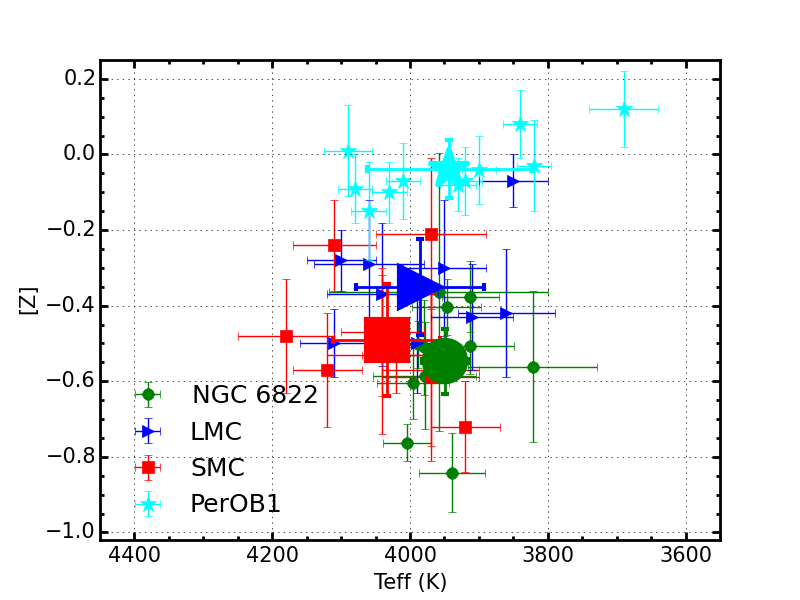
\includegraphics[width=0.65\textwidth]{ngc6822/N6822_TeffvsZ-thesis}
\caption[Effective temperature as a function of metallicity in different environments]{
Effective temperatures as a function of metallicity for four different data sets using the $J$-band analysis technique.
There appears to be no significant variation in the temperatures of RSGs over a range of 0.55 dex.
These results are compiled from the LMC, SMC
\protect\citep[blue and red points respectively;][]{2015ApJ...806...21D}, PerOB1
\protect\citep[a Galactic RSG cluster; cyan;][]{2014ApJ...788...58G} and NGC\,6822 (green).
Mean values for each data set are shown as enlarged points in the same style and colour.
The x-axis is reversed for comparison with Figure~\ref{fig:HRD}.\label{fig:TvsZ}
         }
\end{figure}

\begin{figure}
 \centering
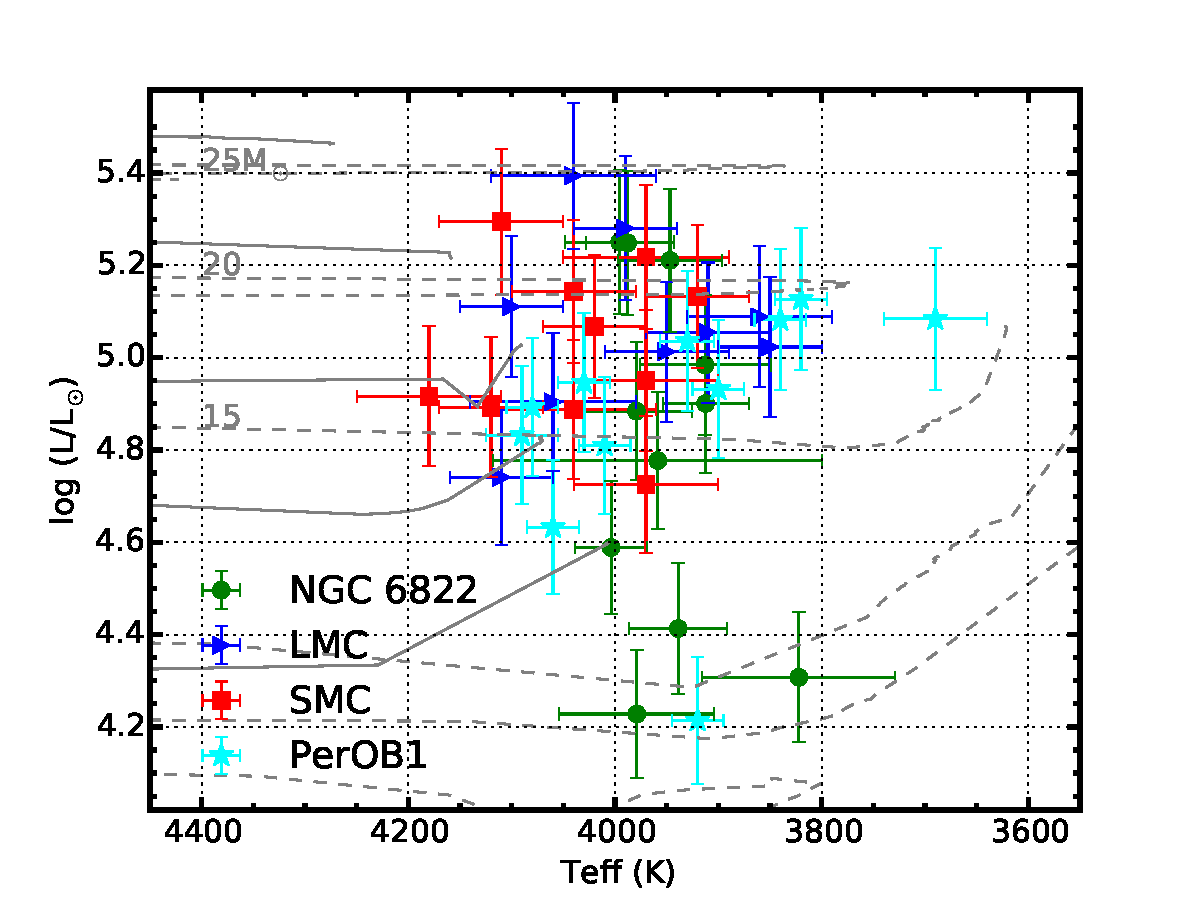
\includegraphics[width=0.65\textwidth]{ngc6822/N6822_HRD_all_thesis}
\caption[H-R diagram from four different environments]{
H-R diagram for RSGs in PerOB1 (cyan), LMC (blue), SMC (red) and NGC\,6822 (green) which have stellar parameters obtained using the $J$-band method.
This figure shows that there appears to be no significant temperature differences between the four samples.
Solid grey lines show SMC-like metallicity evolutionary models including rotation
\protect\citep{2013A&A...558A.103G}.
Dashed grey lines show solar metallicity evolutionary models including rotation
\protect\citep{2012A&A...537A.146E}.\label{fig:HRD}
        }
\end{figure}


From these figures, we see no evidence for significant variations in the average temperatures of RSGs with respect to metallicity.
This is in contrast to current evolutionary models which display a change of $\sim$~450K,
for a M~=~15\,M$_{\odot}$ model,
over a range of solar to SMC-like metallicities~\citep{2012A&A...537A.146E,2013A&A...558A.103G}.

For solar metallicity, observations in PerOB1 are in good agreement with the models
\citep[see Figure 9 in][]{2014ApJ...788...58G}.
However, at SMC-like metallicity, the end-points of the models are systematically warmer than the observations.
The temperature of the end-points of the evolutionary models of massive stars could depend on the choice of the convective mixing-length parameter
\citep{1992A&AS...96..269S}.
That the models produce a higher temperature than observed could imply that the choice of a solar-like mixing-length parameter does not hold for higher-mass stars at lower metallicity.

Lastly, we note that the average spectral type of RSGs tends towards an earlier spectral type with decreasing metallicity over this range
\citep{1979ApJ...231..384H,2012AJ....144....2L}.
Following the arguments in~\citet{1979ApJ...231..384H} this is not in contradiction to the above results.
Spectral types are measured for RSGs using the optical TiO band-heads at
$\sim$~0.65\,$\mu$m,
whereas in this study temperatures are estimated using near-IR atomic features
(as well as the line-free pseudo-continuum).
The strengths of TiO bands are dependent upon metallicity which means that
the spectral classification for RSGs at a constant temperature will differ
\citep{2013ApJ...767....3D}.
Therefore, although historically spectral type has been used as a proxy for temperature, this assumption does not provide an accurate picture for RSGs.

% Recently,
% \cite{2013ApJ...767....3D} showed that the strength of TiO bands are dependent upon metallicity and that at lower metallicity, the TiO bands are significantly weaker.
% The trend in spectral type (or strength of the TiO absorption features) can be naturally explained by the decreasing abundance of the TiO molecule in lower metallicity environments.

% subsection temperatures_of_rsgs (end)
\subsection{AGB Contamination} % (fold)
\label{sub:AGB_contamination}
As mentioned in Section~\ref{sub:target_selection}, massive AGB stars are potential contaminants to our sample.
These stars have similar properties to RSGs and can occupy similar mass ranges as lower-mass RSGs
\citep{2005ARA&A..43..435H},
however, their lifetimes are around $\sim$\,25\,Myr
\citep{2010MNRAS.401.1453D}.
\cite{1983ApJ...272...99W} argued for an AGB luminosity limit
(owing to the limit on the mass of the degenerate core) of M$_{bol}\sim -$7.1.
Using this maximum luminosity, corrected for the distance to NGC\,6822,
yields $K$~=~14.0.
Four of our analysed stars have $K$-band magnitudes fainter than this limit,
but excluding the results for these does not significantly alter any of our conclusions
(and arguably, they would still be tracing the young stellar population).

% subsection AGB_contamination (end)
% section discussion (end)

\section{Conclusions} % (fold)
\label{sec:conclusions}

KMOS spectroscopy of red supergiant stars (RSGs) in NGC\,6822 is presented.
The data were telluric corrected in two different ways and the standard 3 arm telluric method is shown to work as effectively (in most cases) as the more time expensive 24 arm telluric method.
Radial velocities of the targets are measured and are shown to be consistent with previous results in NGC\,6822, confirming their extragalactic nature.

Stellar parameters are calculated for 11 RSGs using the $J$-band analysis method outlined in
\cite{2010MNRAS.407.1203D}.
The average metallicity within NGC\,6822 is
$\bar{\rm Z}$~=~$-0.55\pm0.13\,dex$,
consistent with previous abundance studies of young stars.
We find an indication of a metallicity gradient within the central 1\,kpc,
however with a low significance caused by the small size and limited spatial extent of our RSG sample.
To conclusively assess the presence of a metallicity gradient among the young population within NGC\,6822 a larger systematic study of RSGs is needed.

The chemical abundances of the young and old stellar populations of NGC\,6822 are well explained by a simple closed-box chemical evolution model.
However, while an interesting result, we note that the closed-box model is unlikely to be a good assumption for this galaxy given its morphology.

The effective temperatures of RSGs in this study are compared to those of all RSGs analysed using the same method.
Using results which span 0.55\,$dex$ in metallicity (Solar to SMC) within four galaxies, we find no evidence for a systematic variation in average effective temperature with respect to metallicity.
This is in contrast with evolutionary models which, for a  similar change in metallicity, produces a shift in the temperature of RSGs of up to 450\,K.
We argue that an observed shift in average spectral type of RSGs over this metallicity range does not imply a shift in average temperature.

% These observations were taken as part of the KMOS Science Verification programme.
% With guaranteed time observations we have obtained data for RSGs in NGC\,300 and NGC\,55 at distances of $\sim$1.9\,Mpc,
% as well as observations of super-star clusters in M\,83 and the Antennae galaxy at 4.5 and 20\,Mpc, respectively.
% Owing to the fact that RSGs dominate the light output from super-star clusters
% \citep{2013MNRAS.430L..35G} these clusters can be analysed in a similar manner
% \citep{2014ApJ...787..142G},
% which will provide metallicity measurements at distances a factor of 10 larger than using individual RSGs!
% This work is the first step towards an ambitious proposal to survey a large number of galaxies in the Local Volume,
% motivated by the twin goals of investigating their abundance patterns,
% while also calibrating the relationship between galaxy mass and metallicity in the Local Group.

% section conclusions (end)


% \subsection{Telluric Correction}
% \label{sub:Telluric Corrections}

% One of the most important stages within the data reduction process, for our science, is the correction for the effects of the Earth's atmosphere.
% As starlight passes through the atmosphere it is absorbed and re-emitted by various different molecules.
% These strong molecular features contaminate and blend genuine stellar features.
% In order to recover the stellar features a spectrum is derived which contains only the atmospheric absorption features.
% This spectrum is then used to correct the science spectrum.
% % To illustrate this I could show a plot of the transmission model in the near-IR

% Typically, one generates a telluric spectrum by observing an additional star of known spectral type.
% If the stellar features are well characterised for this spectral type, any additional features are assumed to be owing to the Earth's atmosphere.
% The spectral type is usually chosen to minimize the number of stellar features present in the region of interest.
% In the $J$-band an A0V star has few lines of note and is therefore a good choice of telluric standard star in this regime.
% % Show a plot of an A0V star in the near-IR
% This method of telluric correction is robust and well tested, however, it does have some fairly fundamental limitations.
% These limitations include the fact that it is impossible to sample precisely the same atmospheric column in both the science and telluric observations, as well as the additional time it takes to observe a standard star.

% Recently, a tool for telluric correction which does not use standard star observations has been developed and tested on some VLT instruments~\citep{molecfit}.
% This package uses atmospheric modelling techniques to derive a telluric spectrum.
% The package is briefly explained in section~\ref{sub:molecfit}, however, see ~\cite{molecfit} for a more thorough description.

% \subsubsection{Standard Star Telluric Correction} % (fold)
% \label{sub:standard_star_telluric_correction}

% % Intro.
% In normal KMOS observing mode, the standard template for telluric observations is to observe one telluric standard star in an IFU on each of the three KMOS spectrographs.
% However, there is an alternative template which allows users to observe one standard star in each of the 24 KMOS IFUs rather than each detector.
% This strategy provides a more accurate telluric correction for most of the KMOS IFUs however it does reduce observing efficiency.
% In order to quantify the difference between these two methods and to determine if the more rigorous telluric observation is required, for these observations a telluric standard star (HIP97618) was observed in each of the 24 KMOS IFUs.
% This gave us the tools with which to check both telluric correction routines on one data set and to directly compare the two results.

% The reason that these two methods of telluric correction differ is owing to the intrinsic differences between each of the KMOS IFUs as well as the differences between the patch of sky which each IFU observes.
% With respect to the intrinsic differences between the IFUs, the KMOS/esorex pipeline uses flatfield exposures to account for these differences in their \textquoteleft kmo\_illumination\textquoteright ~recipe.
% % To complicate matters, the telluric observations between the IFUs are not identical.
% % This could be down to a number of factors, for example, the sky subtraction between the IFUs is more accurate in some  instances.
% A comparison between the two methods in the H-band is made by
% \cite{2013A&A...558A..56D}, these authors conclude that using the more time efficient telluric correction method is suitable for most science purposes.
% However, an equivalent analysis in the YJ-band is not in the literature.

% % What does the pipeline do?
% The way in which the KMOS/esorex pipeline performs the telluric correction is identical between the two methods.
% The only difference is the number of telluric spectra which are used to perform the corrections.
% The pipeline derives a telluric spectrum using various look-up tables as well as a telluric standard star (of spectral type O, B, A or G) to create a spectrum containing atmospheric absorption features only, where the stellar absorption features (arising from the standard star) have been removed.
% In order to identify the which features are stellar and which are atmospheric, the pipeline references an atmospheric transmission model which it uses to identify the position (in wavelength space) of all of the atmospheric absorption features in this wavelength regime.
% The standard star spectrum is divided by this atmospheric transmission model. %, an example of which can be seen in figure~\ref{...}.
% Any features which remain are assumed to be intrinsic to the standard star.
% These lines are then fit with a Lorentzian profile and subtracted.
% The atmospheric transmission model is then multiplied back into the data.
% The resulting spectrum is now corrected for the intrinsic shape of the telluric standard star using a look-up table of effective temperatures, defined by the luminosity class of the standard star.
% Finally, the spectrum is normalised and the result is the final telluric spectrum.


% \bibliography{../journals}
